\documentclass[11pt,a4paper,dvipsnames]{article}
\usepackage[deliverable]{IOHKCoverPage}


\usepackage[margin=2.5cm]{geometry}
\usepackage{iohk}
\usepackage{microtype}
\usepackage{mathpazo} % nice fonts
\usepackage{amsmath}
\usepackage{amssymb}
\usepackage{amsthm}
\usepackage{latexsym}
\usepackage{mathtools}
\usepackage{stmaryrd}
\usepackage{extarrows}
\usepackage{slashed}
\usepackage[colon]{natbib}
\usepackage[unicode=true,pdftex,pdfa,colorlinks=true]{hyperref}
\usepackage{xcolor}
\usepackage[capitalise,noabbrev,nameinlink]{cleveref}
\usepackage{float}
\floatstyle{boxed}
\restylefloat{figure}
\usepackage{tikz}
\usepackage{booktabs}
\usepackage{enumerate}
\usepackage{comments} \newcommand{\khcomment}[1]{\comment{KH}{#1}}


%%
%% Package `semantic` can be used for writing inference rules.
%%
\usepackage{semantic}
%% Setup for the semantic package
\setpremisesspace{20pt}

% data for Deliverable header -- added by KH from an EU H2020 project template
\DeliverableNumber{GL-D2}
\DeliverableTitle{A Formal Specification of the Cardano Ledger integrating Plutus Core}{Formal Spec: Cardano Ledger with Plutus Core}
\DeliverableResponsible{Formal Methods Team}
\EditorName{Andre Knispel, \IOHK}
\Authors{
   Andre Knispel \quad \texttt{andre.knispel@iohk.io}\\
   Polina Vinogradova \quad \texttt{polina.vinogradova@iohk.io}
   % I think Andre is the main author of this document?  KH
}
\DueDate{28$^{\textrm{th}}$ February 2021}
\SubmissionDate{}{}
\LeaderName{Philipp Kant, \IOHK}
\InstitutionAddress{\IOHK}
\Version{FS-2.2.0}
\Project{Goguen Ledger}
\DisseminationDR

%%
%% Types
%%
\newcommand{\Nothing}{\ensuremath{\Diamond}}
\newcommand{\N}{\ensuremath{\mathbb{N}}}
\newcommand{\Bool}{\type{Bool}}
\newcommand{\Npos}{\ensuremath{\mathbb{N}^{+}}}
\newcommand{\Z}{\ensuremath{\mathbb{Z}}}
\newcommand{\R}{\ensuremath{\mathbb{R}}}
\newcommand{\Rnn}{\ensuremath{\mathbb{R}^{\geq 0}}}
\newcommand{\Tx}{\type{Tx}}
\newcommand{\ShelleyTx}{\type{ShelleyTx}}
\newcommand{\GoguenTx}{\type{GoguenTx}}
\newcommand{\TxBody}{\type{TxBody}}
\newcommand{\UnsignedData}{\type{UnsignedData}}
\newcommand{\VldSR}{\type{VldSR}}
\newcommand{\VldOut}{\type{VldOut}}
\newcommand{\Vlds}{\type{Vlds}}
\newcommand{\TxWitness}{\type{TxWitness}}
\newcommand{\Ix}{\type{Ix}}
\newcommand{\RdmrPtr}{\type{RdmrPtr}}
\newcommand{\TxId}{\type{TxId}}
\newcommand{\Addr}{\type{Addr}}
\newcommand{\UTxO}{\type{UTxO}}
\newcommand{\UTxOIn}{\type{UTxOIn}}
\newcommand{\Wdrl}{\type{Wdrl}}
\newcommand{\Coin}{\type{Coin}}
\newcommand{\PParams}{\type{PParams}}
\newcommand{\ShelleyPParams}{\type{ShelleyPParams}}
\newcommand{\NewParams}{\type{NewParams}}
\newcommand{\Slot}{\type{Slot}}
\newcommand{\MemoryEstimate}{\type{MemoryEstimate}}
\newcommand{\UTCTime}{\type{UTCTime}}
\newcommand{\SlotsPrior}{\ensuremath{\mathsf{SlotsPrior}}}
\newcommand{\SlotsPerEpoch}{\mathsf{SlotsPerEpoch}}
\newcommand{\SlotsPerKESPeriod}{\mathsf{SlotsPerKESPeriod}}
\newcommand{\SlotsStabilityParam}{\fun{k}}
\newcommand{\Duration}{\type{Duration}}
\newcommand{\StakePools}{\type{StakePools}}
\newcommand{\StakeDeleg}{\type{StakeDeleg}}
\newcommand{\StakeCreds}{\type{StakeCreds}}
\newcommand{\Seed}{\type{Seed}}
\newcommand{\seedOp}{\star}
\newcommand{\Ppm}{\type{Ppm}}
\newcommand{\Tppm}{\mathsf{T_{ppm}}}
\newcommand{\Value}{\type{Value}}
\newcommand{\ProtVer}{\ensuremath{\type{ProtVer}}}
\newcommand{\Language}{\type{Language}}
\newcommand{\ApName}{\ensuremath{\type{ApName}}}
\newcommand{\ApVer}{\ensuremath{\type{ApVer}}}
\newcommand{\SystemTag}{\ensuremath{\type{SystemTag}}}
\newcommand{\InstallerHash}{\ensuremath{\type{InstallerHash}}}
\newcommand{\PPUpdate}{\type{PPUpdate}}
\newcommand{\Applications}{\type{Applications}}
\newcommand{\AVUpdate}{\type{AVUpdate}}
\newcommand{\Update}{\type{Update}}
\newcommand{\DCert}{\type{DCert}}
\newcommand{\DCertRegKey}{\type{DCert_{regkey}}}
\newcommand{\DCertDeRegKey}{\type{DCert_{deregkey}}}
\newcommand{\DCertDeleg}{\type{DCert_{delegate}}}
\newcommand{\DCertRegPool}{\type{DCert_{regpool}}}
\newcommand{\DCertRetirePool}{\type{DCert_{retirepool}}}
\newcommand{\DCertGen}{\type{DCert_{genesis}}}
\newcommand{\DCertMir}{\type{DCert_{mir}}}
\newcommand{\PoolParam}{\type{PoolParam}}
\newcommand{\UTxOState}{\ensuremath{\type{UTxOState}}}
\newcommand{\SFState}{\ensuremath{\type{SFState}}}
\newcommand{\ledgerState}{\ensuremath{\type{ledgerState}}}
\newcommand{\ValEnv}{\type{ValEnv}}
\newcommand{\ValState}{\type{ValState}}
\newcommand{\ScrInData}{\type{ScrInData}}
\newcommand{\AddrRWD}{\type{Addr_{rwd}}}
\newcommand{\AddrB}{\type{Addr_{base}}}
\newcommand{\AddrP}{\type{Addr_{ptr}}}
\newcommand{\AddrE}{\type{Addr_{enterprise}}}
\newcommand{\AddrBS}{\type{Addr_{bootstrap}}}
\newcommand{\Ptr}{\type{Ptr}}
\newcommand{\DState}{\type{DState}}
\newcommand{\DWEnv}{\type{DWEnv}}
\newcommand{\DPSEnv}{\type{DPSEnv}}
\newcommand{\DPEnv}{\type{DPEnv}}
\newcommand{\DEnv}{\type{DEnv}}
\newcommand{\PEnv}{\type{PEnv}}
\newcommand{\DPState}{\type{DPState}}
\newcommand{\PState}{\type{PState}}
\newcommand{\DCertBody}{\type{DCertBody}}
\newcommand{\TData}{\type{TData}}
\newcommand{\DPoolReap}{\ensuremath{\type{poolreap}}}
\newcommand{\UPIState}{\type{UPIState}}
\newcommand{\UpdatePayload}{\type{UpdatePayload}}
\newcommand{\NetworkId}{\mathsf{NetworkId}}

% multi-signature
\newcommand{\StakeCredential}{\type{Credential}_{stake}}
\newcommand{\StakeDelegs}{\type{StakeDelegs}}
\newcommand{\Quorum}{\type{Quorum}}

\newcommand{\txwitsVKey}[1]{\fun{txwitsVKey}~\var{#1}}
\newcommand{\txwitsScript}[1]{\fun{txwitsScript}~\var{#1}}

\newcommand{\AddrVKey}{\type{Addr^{vkey}}}
\newcommand{\AddrRWDVKey}{\type{Addr_{rwd}^{vkey}}}
\newcommand{\AddrRWDScr}{\type{Addr_{rwd}^{script}}}
\newcommand{\AddrVKeyB}{\type{Addr^{vkey}_{base}}}
\newcommand{\AddrVKeyP}{\type{Addr^{vkey}_{ptr}}}
\newcommand{\AddrVKeyE}{\type{Addr^{vkey}_{enterprise}}}
\newcommand{\AddrVKeyBS}{\type{Addr^{vkey}_{bootstrap}}}
\newcommand{\AddrScr}{\type{Addr^{script}}}
\newcommand{\AddrScrBase}{\type{Addr_{base}^{script}}}
\newcommand{\AddrScrEnterprise}{\type{Addr_{enterprise}^{script}}}
\newcommand{\AddrScrPtr}{\type{Addr_{ptr}^{script}}}
\newcommand{\AuxiliaryDataHash}{\type{AuxiliaryDataHash}}
\newcommand{\AuxiliaryData}{\type{AuxiliaryData}}
\newcommand{\Metadata}{\type{Metadata}}
\newcommand{\DataHash}{\type{DataHash}}
\newcommand{\TxInfo}{\type{TxInfo}}
\newcommand{\Datum}{\type{Datum}}
\newcommand{\Redeemer}{\type{Redeemer}}
\newcommand{\EpochInfo}{\type{EpochInfo}}
\newcommand{\SystemStart}{\type{SystemStart}}
\newcommand{\ScriptHash}{\type{ScriptHash}}
\newcommand{\PolicyID}{\type{PolicyID}}
\newcommand{\LangDepView}{\type{LangDepView}}
\newcommand{\ScriptIntegrityHash}{\type{ScriptIntegrityHash}}
\newcommand{\Script}{\type{Script}}
\newcommand{\ScriptPlutus}{\type{Script}_{plc}}
\newcommand{\PlutusVI}{\type{PlutusV1}}
\newcommand{\PlutusVII}{\type{PlutusV2}}
\newcommand{\ScriptPhOne}{\type{Script^{ph1}}}
\newcommand{\ScriptPhTwo}{\type{Script^{ph2}}}
\newcommand{\ScriptV}{\type{Script_{v}}}
\newcommand{\ScriptPurpose}{\type{ScriptPurpose}}
\newcommand{\Rdmrs}{\type{Rdmrs}}
\newcommand{\DorR}{\type{DorR}}
\newcommand{\ValidationData}{\type{ValidationData}}
\newcommand{\IsValid}{\type{IsValid}}
\newcommand{\HashUnsData}{\type{HashUnsData}}
\newcommand{\True}{\mathsf{True}}
\newcommand{\False}{\mathsf{False}}
\newcommand{\MSig}{\type{MSig}}
\newcommand{\Tag}{\type{Tag}}
\newcommand{\Credential}{\type{Credential}}
\newcommand{\AssetID}{\type{AssetID}}
\newcommand{\Integer}{\type{Integer}}

%% Adding witnesses
\newcommand{\AssetName}{\type{AssetName}}
\newcommand{\Quantity}{\type{Quantity}}
\newcommand{\TxIn}{\type{TxIn}}
\newcommand{\OutRef}{\type{OutRef}}
\newcommand{\ShelleyTxIn}{\type{ShelleyTxIn}}
\newcommand{\ShelleyTxOut}{\type{ShelleyTxOut}}
\newcommand{\ShelleyUTxO}{\type{ShelleyUTxO}}
\newcommand{\ShelleyChainState}{\type{ShelleyChainState}}
\newcommand{\HasDV}{\type{HasDV}}
\newcommand{\TxInScr}{\type{TxInScr}}
\newcommand{\Info}{\type{Info}}
\newcommand{\ExUnits}{\type{ExUnits}}
\newcommand{\CostMod}{\type{CostModel}}
\newcommand{\ByteString}{\type{ByteString}}
\newcommand{\ValidityInterval}{\type{ValidityInterval}}
\newcommand{\Network}{\type{Network}}
\newcommand{\Prices}{\type{Prices}}
\newcommand{\IsFee}{\type{IsFee}}
\newcommand{\TxOut}{\type{TxOut}}
\newcommand{\OutFoo}{\type{OutFoo}}
\newcommand{\VKey}{\type{VKey}}
\newcommand{\VKeyEv}{\type{VKey_{ev}}}
\newcommand{\VKeyGen}{\type{VKey_G}}
\newcommand{\SKey}{\type{SKey}}
\newcommand{\SKeyEv}{\type{SKey_{ev}}}
\newcommand{\KeyHash}{\type{KeyHash}}
\newcommand{\RewardAcnt}{\type{RewardAcnt}}
\newcommand{\KeyHashGen}{\type{KeyHash_G}}
\newcommand{\KeyPair}{\type{KeyPair}}
\newcommand{\KeyPairEv}{\type{KeyPair_{ev}}}
\newcommand{\Sig}{\type{Sig}}
\newcommand{\Data}{\type{Data}}
%% Adding delegation
\newcommand{\Epoch}{\type{Epoch}}
\newcommand{\KESPeriod}{\type{KESPeriod}}
%% Blockchain
\newcommand{\Gkeys}{\var{G_{keys}}}
\newcommand{\Block}{\type{Block}}
\newcommand{\SlotId}{\type{SlotId}}
\newcommand{\PPUpdateEnv}{\type{PPUpdateEnv}}
\newcommand{\AVUpdateEnv}{\type{AVUpdateEnv}}
\newcommand{\AVUpdateState}{\type{AVUpdateState}}
\newcommand{\UpdateEnv}{\type{UpdateEnv}}
\newcommand{\UpdateState}{\type{UpdateState}}
\newcommand{\UTxOEnv}{\type{UTxOEnv}}
\newcommand{\CEEnv}{\type{CEEnv}}
\newcommand{\CEState}{\type{CEState}}
\newcommand{\BDEnv}{\type{BDEnv}}
\newcommand{\BDState}{\type{BDState}}
\newcommand{\LEnv}{\type{LEnv}}
\newcommand{\LState}{\type{LState}}
\newcommand{\GoguenChainState}{\type{GoguenChainState}}
%%
%% Functions
%%
\newcommand{\txins}[1]{\fun{txins}~ \var{#1}}
\newcommand{\txouts}[1]{\fun{txouts}~ \var{#1}}
\newcommand{\txcerts}[1]{\fun{txcerts}~ \var{#1}}
\newcommand{\txid}[1]{\fun{txid}~ \var{#1}}
\newcommand{\outs}[1]{\fun{outs}~ \var{#1}}
\newcommand{\values}[1]{\fun{values}~ #1}
\newcommand{\ubalance}[1]{\fun{ubalance}~ \var{#1}}
\newcommand{\txttl}[1]{\fun{txttl}~ \var{#1}}
\newcommand{\firstSlot}[1]{\fun{firstSlot}~ \var{#1}}
\newcommand{\deposited}[2]{\fun{deposited}~ \var{#1} ~ \var{#2}}
\newcommand{\decayedKey}[4]{\fun{decayedKey}~ \var{#1}~ \var{#2}~ \var{#3}~ \var{#4}}
\newcommand{\decayedTx}[3]{\fun{decayedTx}~ \var{#1}~ \var{#2}~ \var{#3}}
\newcommand{\keyRefund}[6]{\fun{keyRefund}~ {#1}~{#2}~{#3}~\var{#4}~\var{#5}~\var{#6}}
\newcommand{\refund}[4]{\fun{refund}~ \var{#1}~ \var{#2}~ {#3}~ {#4}}
\newcommand{\keyRefunds}[2]{\fun{keyRefunds}~ \var{#1}~ \var{#2}}
\newcommand{\consumed}[4]{\fun{consumed}~ \var{#1}~ \var{#2}~ \var{#3}~ \var{#4}}
\newcommand{\produced}[2]{\fun{produced}~ \var{#1}~ \var{#2}}
\newcommand{\applyFun}[2]{\fun{#1}~\var{#2}}

\newcommand{\RegKey}[1]{\textsc{RegKey}(#1)}
\newcommand{\DeregKey}[1]{\textsc{DeregKey}(#1)}
\newcommand{\Delegate}[1]{\textsc{Delegate}(#1)}
\newcommand{\RegPool}[1]{\textsc{RegPool}(#1)}
\newcommand{\RetirePool}[1]{\textsc{RetirePool}(#1)}
\newcommand{\cwitness}[1]{\fun{cwitness}~ \var{#1}}
\newcommand{\dpool}[1]{\fun{dpool}~ \var{#1}}
\newcommand{\poolParam}[1]{\fun{poolParam}~ \var{#1}}
\newcommand{\retire}[1]{\fun{retire}~ \var{#1}}
\newcommand{\addrRw}[1]{\fun{addr_{rwd}}~ \var{#1}}
\newcommand{\epoch}[1]{\fun{epoch}~\var{#1}}
\newcommand{\kesPeriod}[1]{\fun{kesPeriod}~\var{#1}}
\newcommand{\pps}[1]{\fun{pps}~ \var{#1}}

%% UTxO witnesses
\newcommand{\inputs}[1]{\fun{inputs}~ \var{#1}}
\newcommand{\txwits}[1]{\fun{txwits}~ \var{#1}}
\newcommand{\verify}[3]{\fun{verify} ~ #1 ~ #2 ~ #3}
\newcommand{\sign}[2]{\fun{sign} ~ #1 ~ #2}
\newcommand{\verifyEv}[4]{\fun{verify_{ev}} ~ #1 ~ #2 ~ #3 ~ #4}
\newcommand{\signEv}[3]{\fun{sign_{ev}} ~ #1 ~ #2 ~ #3}
\newcommand{\serialised}[1]{\llbracket \var{#1} \rrbracket}
\newcommand{\hashKey}[1]{\fun{hashKey}~ \var{#1}}
\newcommand{\txbody}[1]{\fun{txbody}~ \var{#1}}
\newcommand{\txfee}[1]{\fun{txfee}~ \var{#1}}
\newcommand{\txwdrls}[1]{\fun{txwdrls}~ \var{#1}}
\newcommand{\minfee}[2]{\fun{minfee}~ \var{#1}~ \var{#2}}
\newcommand{\slotminus}[2]{\var{#1}~-_{s}~\var{#2}}
\DeclarePairedDelimiter\floor{\lfloor}{\rfloor}
% wildcard parameter
\newcommand{\wcard}[0]{\underline{\phantom{a}}}
%% Adding ledgers...
\newcommand{\utxo}[1]{\fun{utxo}~ #1}
%% Delegation
\newcommand{\delegatesName}{\fun{delegates}}
\newcommand{\delegates}[3]{\delegatesName~#1~#2~#3}
\newcommand{\dwho}[1]{\fun{dwho}~\var{#1}}
\newcommand{\depoch}[1]{\fun{depoch}~\var{#1}}
\newcommand{\dval}{\ensuremath{d_{\mathsf{val}}}}
%% Delegation witnesses
\newcommand{\dbody}[1]{\fun{dbody}~\var{#1}}
\newcommand{\dwit}[1]{\fun{dwit}~\var{#1}}
%% Blockchain
\newcommand{\bwit}[1]{\fun{bwit}~\var{#1}}
\newcommand{\bslot}[1]{\fun{bslot}~\var{#1}}
\newcommand{\bbody}[1]{\fun{bbody}~\var{#1}}
\newcommand{\bhbody}[1]{\fun{bhbody}~\var{#1}}
\newcommand{\bdlgs}[1]{\fun{bdlgs}~\var{#1}}
%% ledgerstate constants
\newcommand{\genesisId}{\ensuremath{Genesis_{Id}}}
\newcommand{\genesisTxOut}{\ensuremath{Genesis_{Out}}}
\newcommand{\genesisUTxO}{\ensuremath{Genesis_{UTxO}}}
\newcommand{\genesisUTxOState}{(\genesisUTxO,\wcard,\wcard,\wcard)}
\newcommand{\emax}{\ensuremath{\mathsf{E_{max}}}}

\newcommand{\unitInterval}{\ensuremath{[0,~1]}}
\newcommand{\unitIntervalNonNull}{\ensuremath{(0,~1]}}
\newcommand{\nonnegReals}{\ensuremath{[0,~\infty)}}
\newcommand{\posReals}{\ensuremath{(0,~\infty)}}

\newcommand{\Val}{\fun{Val}}
\newcommand{\Utxo}{\fun{Utxo}}
\newcommand{\field}{\fun{field}}


\theoremstyle{definition}
\newtheorem{definition}{Definition}[section]
\newtheorem{property}{Property}[section]
\newtheorem{lemma}[definition]{Lemma}
\newtheorem{theorem}[definition]{Theorem}
\newtheorem{corollary}[definition]{Corollary}

\newcommand{\leteq}{\ensuremath{\mathrel{\mathop:}=}}

\definecolor{hldiffcolor}{rgb}{0.95, 0.93, 0}
\newcommand{\hldiff}[1]{\mathchoice
  {\colorbox{hldiffcolor}{$\displaystyle#1$}}
  {\colorbox{hldiffcolor}{$\textstyle#1$}}
  {\colorbox{hldiffcolor}{$\scriptstyle#1$}}
  {\colorbox{hldiffcolor}{$\scriptscriptstyle#1$}}}
\DeclareMathOperator{\supp}{supp}

%% In-para enumeration -- KH
\usepackage{paralist}

%% Enumeration args -- KH
\usepackage{enumitem}

\begin{document}

\hypersetup{
  pdftitle={Design of the Cardano Ledger with Automated Parameter Updates},
  breaklinks=true,
  bookmarks=true,
  colorlinks=false,
  linkcolor={blue},
  citecolor={blue},
  urlcolor={blue},
  linkbordercolor={white},
  citebordercolor={white},
  urlbordercolor={white}
}


\floatstyle{boxed}
\restylefloat{figure}
\cleardoublepage
\renewcommand{\thepage}{\arabic{page}}
\setcounter{page}{1}

\title{Design of the Cardano Ledger with Automated Parameter Updates and Central Fund Transfers}

\author{
   Kevin Hammond \\ {\small \texttt{kevin.hammond@iohk.io}} \\
   Philipp Kant \\ {\small \texttt{philipp.kant@iohk.io}} \\
   Andre Knispel \\ {\small \texttt{andre.knispel@iohk.io}} \\
   }

\date{}

\maketitle

\begin{abstract}
  This document outlines the design of the mechanisms that are needed to support
  automated parameter updates and central funds transfers (collectively PUP).  The PUP mechanism enables a key part of the Cardano governance structure by
  eliminating the use of genesis keys or delegates to control the operation of the Cardano blockchain.  This enables decentralised governance of the blockchain.
  The overall governance process includes both
  off-chain and on-chain components.  This design document is concerned primarily with the on-chain component, but also references the corresponding off-chain
  process, and discusses how the two components interact to ensure decentralised governance.  It covers all parts of the on-chain process including proposal submission,
  vote delegation, on-chain voting/endorsement and automated enactment of proposals.
\end{abstract}

\section*{List of Contributors}
\label{acknowledgements}

\begin{changelog}
\change{2021-02-16}{Kevin Hammond}{FM (IOHK)}{Initial version. }
\change{2021-02-17}{Kevin Hammond}{FM (IOHK)}{Description of goals and submission process.}
\change{2021-02-19}{Kevin Hammond}{FM (IOHK)}{Groups involved.  Vote delegation.}
\change{2021-02-19}{Kevin Hammond}{FM (IOHK)}{Added various outline sections.  Voting, sidechains, short Priviledge comparison.}
\change{2021-02-22}{Kevin Hammond}{FM (IOHK)}{Added workflows, plus textual improvements.}
\change{2021-02-25}{Kevin Hammond}{FM (IOHK)}{Added transition process, updated diagrams, described endorsement and enactment, cleaned up text.}
\change{2021-03-01}{Kevin Hammond}{FM (IOHK)}{Reviewed and updated text.  Added missing diagram, section on transition.}
\change{2021-03-03}{Kevin Hammond}{FM (IOHK)}{Added appendix on user experience.}
\change{2021-03-05}{Kevin Hammond}{FM (IOHK)}{Revised and tidied.  Added address structure and other diagrams.  Checked against delegation design document.}
\change{2021-03-10}{Kevin Hammond}{FM (IOHK)}{Clarified automated endorsement.  Decision needs to be taken on whether endorsement is stake-based or block-based.}
\change{2021-03-12}{Kevin Hammond}{FM (IOHK)}{Added appendix on protocol parameters.  Updated text.}
\change{2021-03-12}{Kevin Hammond}{FM (IOHK)}{Incorporated initial feedback from Andre and Philipp.}
\change{2021-03-15}{Kevin Hammond}{FM (IOHK)}{Added Section on Design Notes to record discussion.}
\change{2021-04-01}{Kevin Hammond}{FM (IOHK)}{Added Appendix on Native Token Governance}
\change{2021-04-01}{Kevin Hammond}{FM (IOHK)}{Added Appendix on Expert Ballots}
\change{2021-04-09}{Kevin Hammond}{FM (IOHK)}{Added Section on Differentiated Submission Groups}
\end{changelog}



\tableofcontents
\listoffigures

\section{Introduction}

The aim of this design is to eliminate the use of the genesis keys (or delegates) within the formal ledger rules.  This will enable
decentralised governance of the blockchain protocol by supporting automated submission and enactment of proposals (PUP).
The process is designed to meet current and future national and international regulatory concerns by removing control of the blockchain protocol
from a small centralised group of actors.

There are three places where genesis keys are currently used.


\begin{itemize}
\item
  \textbf{Parameter Updates:}
  Any updatable protocol parameter may be changed.  Multiple parameters may be changed as part of a single update proposal.
\item
  \textbf{Protocol Version Changes:}
  A change may be made to a major or minor protocol version (a ``hard fork'').  The change must be accompanied by upgrades to
  the software that is being used by block producing nodes (``stake pools''), and acknowledged by sufficient pools upgrading to the new software version.
\item
  \textbf{Transfers from/to Reserves/Treasury:}
  A funds transfer may be made directly from eiher the reserves or treasury pots to a nomrmal address, between the reserves and treasury pots (in either direction), or from a normal address to the treasury pot.  This is referred to in the existing Cardano documentation as an ``MIR'' transfer (Move Instantaneous Rewards).
\end{itemize}

All of these issues must be devolved to a decentralised governance process.

\subsection{Outline Governance Process}

The proposed governance process involves both off-chain and on-chain components.

\begin{enumerate}
\item
  \textbf{Off-Chain:}
  An issue is discussed off-chain.  A vote is taken on a specific proposal using the Catalyst system.  The proposal must be sufficiently unambiguous that its intention is clear, and must include dates by which the proposal is to be submitted and enacted on chain.
\item
  \textbf{On-Chain:}
  A formal proposal is constructed that captures the intention of the off-chain proposal.  It is submitted, verified, and then enacted on-chain.  The proposal will specify the date at which it will be enacted if it is
  properly accepted and endorsed.
\end{enumerate}


The outline process for enacting a proposal is shown in Figure~\ref{fig:workflows}.   The process is split into two main parts: the initial off-chain process, which is expected to be largely manual; and the second, on-chain process, which will largely be
automated.  Only the latter needs to be captured by formal ledger rules.  In order to establish confidence in the governance process,
it is necessary to link the off-chain and on-chain processes.

\begin{figure}
  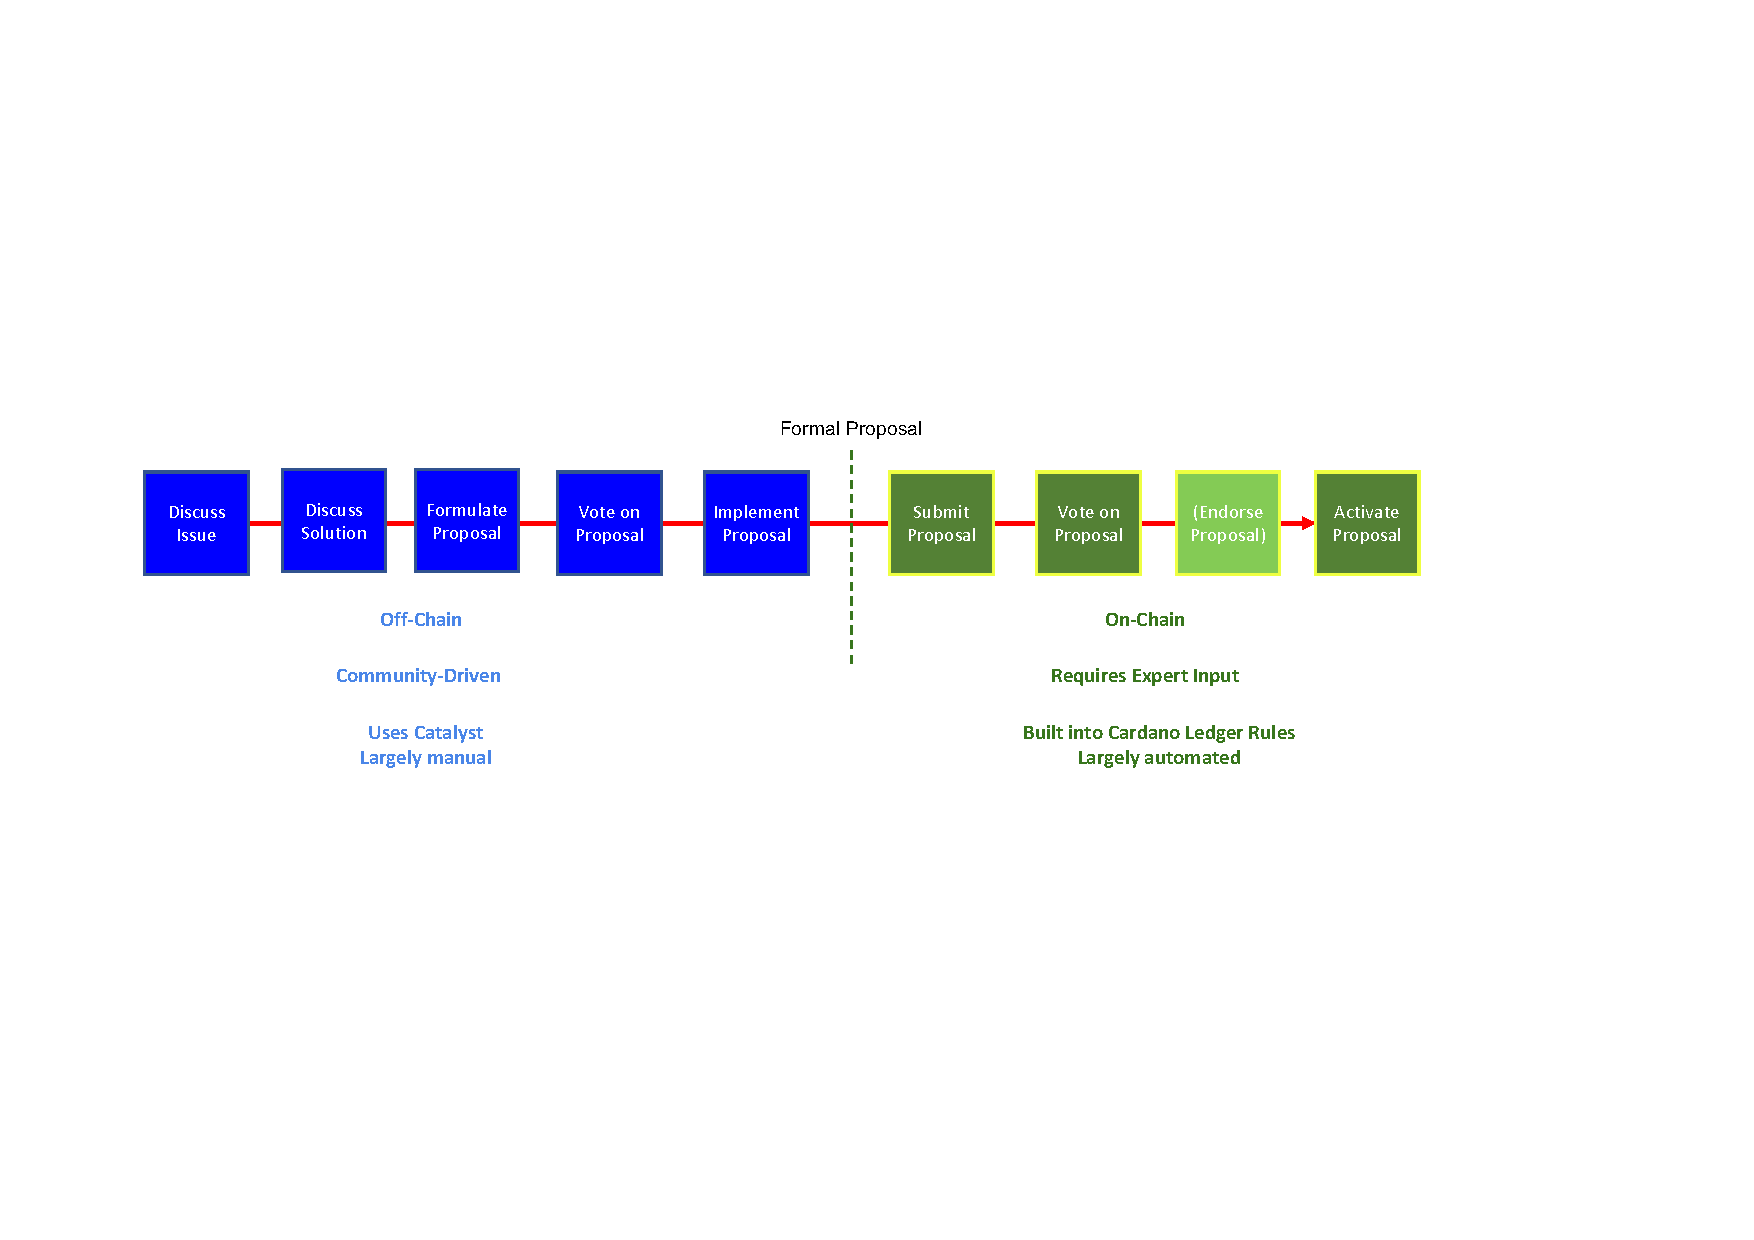
\includegraphics[trim=30 200 100 100,clip,width=\textwidth]{StoryBoard}
  \caption{Outline Process: Ideas are discussed off-chain and voted on using the Catalyst mechanism.  Successful proposals are implemented, and then submitted for on-chain voting and enactment.}
\label{fig:workflows}
\end{figure}


\newpage
\subsection{Off-Chain Process}

The off-chain process involves five key stages:

\begin{enumerate}
\item
  \textbf{Discussion.}  An issue is discussed.  This may be either formal or informal discussion, using a mechanism such as IdeaScale, a community forum such as a TeleGram channel or the Cardano Forum,
  or any other appropriate mechanism.
\item
  \textbf{Ideation.}  A concrete proposal that addresses the issue is formulated by an interested party.
\item
  \textbf{Submission.}  A proposal is submitted for voting.  The submission of proposals must follow the defined process, and may be restricted in some way.
\item
  \textbf{Voting.}  Voters may vote on whether a proposal should be progressed to implementation, requires amendment etc.  Outline or exact deadlines should be agreed as part of this process.
\item
  \textbf{Implementation.}  Accepted proposals are implemented.  For a simple proposal (eg a change to an updatable parameter), this may be as simple as capturing the intentions of the original proposal in a corresponding JSON file.
  Proposals to change protocol versions may involve significant software development, and therefore need to be funded by the Catalyst fund or some other means.
\end{enumerate}

Each of these off-chain stages may follow formally defined processes, and may be partially automated.  Generally, they will be driven by convention and rules.  A detailed governance structure is necessary to ensure that necessary business can
be transacted in an efficient and effective way, without risking loss of control to a small non-representative group, and so negating the purpose of decentralised governance.
The processes and structures may evolve over time.  Some of the issues are discussed in Appendix~\ref{sect:off-chain}.


\newpage
\subsection{On-Chain Process}

Once a proposal has been implemented in the required form, it may be submitted for enactment on-chain.  The on-chain process involves four key stages that are fully automated.  Extreme care needs to be taken with these processes,
since it may not always be possible to stop or reverse actions once they are initiated.

\begin{enumerate}
\item
  \textbf{Submission.}  A formal proposal is submitted on-chain by one of a group of submitters.  The proposal must be in the agreed format, and must include deadlines for voting, endorsement and enactment.
\item
  \textbf{Voting.}  The proposal is voted on and the votes are tallied.  If sufficient votes are obtained by the stated deadline, then the proposal is approved for enactment.
\item
  \textbf{Endorsement.}  If the proposal involves a change to the protocol, then stake pool operators must upgrade their nodes to the correct version.  This will signal their readiness to run the new protocol.
  Assuming that sufficient endorsement is obtained by the deadline, then the proposal is endorsed for enactment.
\item
  \textbf{Enactment.}  Proposals that have been approved (and endorsed, if necessary) are processed fully automatically at the corresponding epoch boundary.
\end{enumerate}

\newpage
\subsection{Key Stakeholder Groups}

A number of stakeholder groups are involved in the governance process.  The key ones are:

\begin{itemize}
\item
  \textbf{Normal Ada Holders:}
  Normal Ada holders are invested in the Cardano ecosystem in financial and other ways.
   In order to ensure fully decentralised governance, the goal of the PUP design is that normal Ada holders should have the ultimate governance power. They may, however, choose to delegate this to specialists when dealing with more technical issues, for example.
%  This ensures fully decentralised governance.
  \item
  \textbf{Stake Pool Operators:}
  Stake pool operators have the responsibility for maintaining the Cardano network.  They are heavily invested in the Cardano ecosystem through the commitment of their time, money and other resources.
  In addition to other voting rights, they need to maintain software compatibility with the latest version of the Cardano blockchain protocol.
  \item
  \textbf{End-Users:}
  These are individuals or organisations who use the Cardano blockchain to process transactions etc.  They may hold minimal ada, perhaps only on a transient basis.
  This will give them limited or no governance rights.  Their needs should, however, be considered when changes are made to protocol parameters.
  \item
  \textbf{Exchanges and other Proxy Ada Holders:}
  Exchanges and similar organisations hold Ada on behalf of other parties.  It is important from both a regulatory and a technical perspective that they do not hold excessive
  power, since this will work against the requirements of decentralisation.  They require a safe, secure and robust blockchain so that they may operate successfully on
  behalf of their clients.
\end{itemize}

The network should be able to evolve in a way that meets the best long-term needs of all these stakeholders, while maintaining the integrity, stability and longevity of
the Cardano blockchain.


\section{Language Versions and Cost Models}
\label{sec:protocol-parameters}

We require the following types (see Figure~\ref{fig:defs:protocol-parameters})
in addition to those that are already defined in the Shelley specification~\cite{shelley_spec}.

\vspace{12pt}
\begin{tabular}{lp{5in}}
  $\Language$ &
  This represents the language name/tag, including the
  version number.
  \\
  $\ExUnits$ &
  A term of this type contains two integer values,
  $(mem, steps)$.
  These represent abstract notions of the relative memory usage and script execution steps,
  respectively.
  \\
  $\CostMod$ &
  A term of this type represents the vector of coefficients that are used to generate
  a term of type $\ExUnits$ given a vector of some resource primitives. The mapping is defined
  concretely by the specific version of the Plutus interpreter that is associated with $\Language$.
  We keep this type as abstract in the specification.
  \\
  $\Prices$ &
  A term of this type comprises two integer values that correspond to the components of $\ExUnits$,
  $\var{(pr_{mem}, pr_{steps})}$:
  $pr_{mem}$ is the price (in Ada) per unit of memory, and $pr_{steps}$ is the price (in Ada) per
  reduction step. This is used to calculate the Ada cost for a specific script execution.
\end{tabular}

\subsection{Language Versions and Backwards Compatibility Requirements}
\label{sec:versions}

In the $\Language$ type, each \emph{version} of a language is considered to be a different language (so there might be several versions of the Plutus language, each of which would be considered to
be different).
Each such language needs to be interpreted by a language-specific interpreter that is called from the ledger implementation.
The interpreter is provided with the (language- and version-specific) arguments that it requires.
It is necessary for the ledger to be capable of executing scripts in all languages it has ever supported.
This implies that it is necessary to maintain all forms of ledger
data that is needed by any past or current language, which constrains future ledger designs.
Introducing a new language will require a protocol version update, since the datatypes need to support the new language and the ledger rules must be updated to use the new interpreter.

\subsection{Determinism of Script Evaluation}
\label{sec:determinism}

The data that is passed to the interpreter
includes the validator script, the redeemer, possibly a datum from the UTxO, information about the transaction that
embeds the script, any relevant ledger data, and any relevant protocol parameters.
It is necessary for the validation outcome of any scripts to remain the same during the entire
period between transaction
submission and completion of the script processing.
%
In order to achieve this,
any data that is passed to the interpreter must be determined by the transaction body itself.
The transaction body therefore includes a hash of any such data that is not uniquely determined by other parts of the transaction body or the UTXO.
When the transaction is processed, as part of the UTXOW rule, this hash is compared with a hash of the data that is passed to the interpreter. This
ensures that scripts are only executed if they have been provided with the intended data.

The $\fun{getLanguageView}$ function (Figure~\ref{fig:defs:protocol-parameters}) filters the data relvant
to a given language from the protocol parameters. Recall here that $\Tppm$ is the type of the
protocol parameter $\var{ppm}~\in~\Ppm$, and that $\PParams~=~\Ppm~\mapsto~\Tppm$.
The type $\LangDepView$ is a subrecord of $\PParams$.
%
At the time of writing, the only parameter that needs to be passed to the $\PlutusVI$
interpreter is the cost model, specifically only the cost model for the $\PlutusVI$ language.

\subsection{Script Evaluation Cost Model and Prices}
\label{sec:cost-mod}

To convert resource primitives into the
more abstract $\ExUnits$ during script execution a cost model needs to be supplied to the interpreter.
The cost models required for this purpose are recorded in the $\var{costmdls}$ protocol parameter.
%
The calculation of the actual cost, in Ada, of running
a script that takes $\var{exunits} \in \ExUnits$ resources to run,
is done by a formula in the ledger rules, which uses the
$\var{prices}$ parameter. This is a parameter that applies to all
scripts and that cannot be varied for individual languages. This parameter
reflects the real-world costs in terms of energy usage, hardware resources etc.

In Alonzo, the protocol parameter $\var{minUTxOValue}$ is deprecated, and replaced by
$\var{coinsPerUTxOWord}$. This specifies directly the deposit required for storing
bytes of data on the ledger in the form of UTxO entries.

\textbf{Limiting Script Execution Costs.}
The $\var{maxTxExUnits}$ and $\var{maxBlockExUnits}$ protocol parameters are
used to limit the total per-transaction and per-block resource use. These only apply to non-native scripts.
The parameters are used to ensure that the time and memory that are required to verify a block are bounded.

\textbf{Value size limit as a protocol parameter.}
The new parameter $\var{maxValSize}$ replaces the constant $\mathsf{maxValSize}$
used (in the ShelleyMA era) to limit the size of the the $\Value$ part of an output in a
serialised transaction.

\textbf{Collateral inputs.}
Collateral inputs in a transaction are used to cover the transaction fees in the case
that a non-native script fails (see Section~\ref{sec:transctions}).
The term \emph{collateral} refers to the total ada contained in the UTxOs referenced 
by collateral inputs.

The parameter $\var{collateralPercent}$ is used to specify the percentage of
the total transaction fee its collateral must (at minimum) cover. The
collateral inputs must not themselves be locked by a script. That is, they must
be VK inputs. The parameter $\var{maxCollInputs}$ is used to limit, additionally,
the total number of collateral inputs, and thus the total number of additional
signatures that must be checked during validation.

\begin{figure*}[htb]
  \emph{Abstract types}
  %
  \begin{equation*}
    \begin{array}{r@{~\in~}l@{\qquad\qquad\qquad}r}
      \var{cm} & \CostMod & \text{Coefficients for the cost model}
    \end{array}
  \end{equation*}
  %
  \emph{Derived types}
  \begin{equation*}
    \begin{array}{r@{~\in~}l@{\quad=\quad}l@{\qquad}r}
      \var{lg}
      & \Language
      & \{\PlutusVI, \dotsb\}
      & \text{Script Language}
      \\
      \var{(pr_{mem}, pr_{steps})}
      & \Prices
      & \Coin \times \Coin
      & \text {Coefficients for $\ExUnits$ prices}
      \\
      \var{(mem, steps)}
      & \ExUnits
      & \N \times \N
      & \text{Abstract execution units}
      \\
      \var{ldv}
      & \LangDepView
      & \Ppm~\mapsto~\Tppm
      & \text{PParams view}
    \end{array}
  \end{equation*}
  %
  \emph{Deprecated Protocol Parameters}
  %
  \begin{equation*}
      \begin{array}{r@{~\in~}l@{\qquad}r}
        \var{minUTxOValue} \mapsto \Coin & \PParams & \text{Min. amount of ada each UTxO must contain}
      \end{array}
  \end{equation*}
  %
  \emph{New Protocol Parameters}
  %
  \begin{equation*}
      \begin{array}{r@{~\in~}l@{\qquad}r}
        \var{costmdls} \mapsto (\Language \mapsto \CostMod) & \PParams \\
        % & \text{Script exec. cost model}\\
        \var{prices} \mapsto \Prices & \PParams \\
        % & \text{Coefficients for $\ExUnits$ prices} \\
        \var{maxTxExUnits} \mapsto \ExUnits & \PParams \\
        % & \text{Max. total tx script exec. resources}\\
        \var{maxBlockExUnits} \mapsto \ExUnits & \PParams \\
        % & \text{Max. total block script exec. resources}\\
        \var{maxValSize} \mapsto \N & \PParams \\
        % & \text{Max size a value can be}\\
        \var{coinsPerUTxOWord} \mapsto \Coin & \PParams \\
        % & \text{Min. lovelace per word (8 bytes) a UTxO entry must contain}
        \var{collateralPercent} \mapsto \N & \PParams \\
        % & \text{Percentage of Tx fee which collateral must cover}
        \var{maxCollInputs} \mapsto \N & \PParams \\
        % & \text{Maximum number of VK inputs that can be used to cover collateral}
      \end{array}
  \end{equation*}
  %
  \emph{Accessor Functions}
  %
  \begin{center}
  \fun{costmdls},~\fun{maxTxExUnits},~\fun{maxBlockExUnits},~\fun{prices}
  \end{center}
  %
  \emph{Helper Functions}
  %
  \begin{align*}
    & \fun{getLanguageView} \in \PParams \to \Language \to \LangDepView \\
    & \fun{getLanguageView}~\var{pp}~\PlutusVI = \var{costmdls}~\mapsto~ (\fun{costmdls}~{pp}~\{\PlutusVI\})
  \end{align*}
  %
  \caption{Definitions Used in Protocol Parameters}
  \label{fig:defs:protocol-parameters}
\end{figure*}


\section{Transactions}
\label{sec:transactions}

This section outlines the changes that are needed to the transaction
structure to enable phase-2 scripts to validate
the minting of tokens, spending outputs, verifying certificates, and
verifying withdrawals.
%
Figure \ref{fig:defs:utxo-shelley-1} gives the modified transaction types and helper functions.
We make the following changes and additions:

\begin{itemize}
  \item $\ScriptIntegrityHash$ is the type of a hash of script execution
  related data. It is the hash of $\fun{txrdmrs}$ and relevant protocol parameters.

  \item $\ScriptPhOne$ is the type of phase-1 scripts.

  \item $\ScriptPhTwo$ is the type of phase-2 scripts.

  \item $\Data$ is a type for communicating data to script.  It is kept abstract here.

  \item $\Script$ is the type of all scripts, both phase-1 and phase-2.

  \item $\IsValid$ is a tag that indicates that a transaction
  expects that all its phase-2 scripts will be validated.
  This tag is added by the block creator when
  constructing a block, and its correctness is verified as part of the script execution.

  \item $\Datum$ is a type alias for the $\Data$ type, used to signify that
  terms of this type are intended to be used strictly as datum objects.

  \item $\Redeemer$ is also a type alias for the $\Data$ type, used to signify that
  terms of this type are intended to be used strictly as redeemers.

  \item $\TxOut$ is the type of transaction outputs. These are extended to include
  an optional hash of a datum. Note that \emph{any} output can
  optionally include such a hash, even though only phase-2 scripts
  can actually use the hash value. Since it is in general impossible for the ledger implementation to
  know at the time of transaction creation whether or not an output belongs to a phase-2
  script, we simply allow any output to contain a hash of a datum.

  \item $\Tag$ lets us differentiate what a script
  can validate, i.e. \\
  \begin{tabular}{l@{~to validate~}l}
  $\mathsf{Spend}$ & spending a script UTxO entry; \\
  $\mathsf{Mint}$ & minting tokens; \\
  $\mathsf{Cert}$  & certificates with script credentials; and  \\
  $\mathsf{Rewrd}$ & reward withdrawals from script addresses.
  \end{tabular}

  \item $\RdmrPtr$ is a pair of a tag and an index. This type is
  used to index the Plutus redeemers that are included in a transaction, as discussed
  below.

\end{itemize}

We add the following helper functions:

\begin{itemize}
  \item $\fun{language}$ selects the language of a phase-2 script, and $\Nothing$ in case
  the script is phase-1.
  \item $\fun{hashData}$ hashes a value of type $\Data$.
  \item $\fun{hashScriptIntegrity}$ hashes the protocol parameters and data relevant to script execution.
  In particular, the redeemer structure, and the datum objects.
\end{itemize}

\begin{figure*}[htb]
  \emph{Abstract types}
  %
  \begin{equation*}
    \begin{array}{l@{\quad\quad\quad\quad}r}
      \ScriptIntegrityHash & \text{Script data hash}\\
      \ScriptPlutus & \text{Plutus core scripts} \\
      \Data & \text{Generic script data}
    \end{array}
  \end{equation*}
  %
  \emph{Script types}
  %
  \begin{equation*}
    \begin{array}{l@{\qquad=\qquad}lr}
      \ScriptPhTwo & \ScriptPlutus \\
      \Script & \ScriptPhOne \uniondistinct \ScriptPhTwo \\
      \IsValid & \Bool \\
      \Datum & \Data \\
      \Redeemer & \Data
    \end{array}
  \end{equation*}
%
  \emph{Derived types}
  %
  \begin{equation*}
    \begin{array}{l@{\qquad=\qquad}lr}
      \ValidityInterval
      & \Slot^? \times \Slot^?
      \\
      \TxOut
      & \Addr \times \Value \times \hldiff{\DataHash^?}
      \\
      \Tag
      & \{\mathsf{Spend},~\mathsf{Mint},~\mathsf{Cert},~\mathsf{Rewrd}\}
      \\
      \RdmrPtr
      & \Tag \times \Ix
    \end{array}
  \end{equation*}
  %
  \emph{Helper Functions}
  %
  \begin{align*}
    \fun{language}& : \Script \to \Language^?\\
    \fun{hashData}& : \Data \to \DataHash
    \nextdef
    \fun{getCoin}& : \TxOut \to \Coin \\
    \fun{getCoin}&~\hldiff{{(\_, \var{v}, \_)}}  = \fun{valueToCoin}~{v}
  \end{align*}
  %
  \begin{align*}
  &\fun{hashScriptIntegrity} : \PParams \to \powerset{\Language} \to (\RdmrPtr \mapsto \Redeemer \times \ExUnits) \\
  &~~~~ \to (\DataHash \mapsto \Datum) \to \ScriptIntegrityHash^? \\
  &\fun{hashScriptIntegrity}~{pp}~{langs}~{rdmrs}~{dats} =  \\
                    &~~~~ \begin{cases}
                          \Nothing & rdmrs = \emptyset \land langs = \emptyset \land dats = \emptyset \\
                          \fun{hash} (rdmrs, dats, \{ \fun{getLanguageView}~pp~l \mid l \in langs \}) & \text{otherwise}
                        \end{cases}
  \end{align*}
  \caption{Definitions for Transactions}
  \label{fig:defs:utxo-shelley-1}
\end{figure*}


\begin{figure*}[htb]
  \emph{Transaction Types}
  %
  \begin{equation*}
    \begin{array}{r@{~~}l@{~~}l@{\qquad}l}
      \TxWitness =
       & (\VKey \mapsto \Sig) & \fun{txwitsVKey} & \text{VKey signatures}\\
       & \times ~(\ScriptHash \mapsto \Script)  & \fun{txscripts} & \text{All scripts}\\
       & \times~ \hldiff{(\DataHash \mapsto \Datum)} & \hldiff{\fun{txdats}} & \text{All datum objects}\\
       & \times ~\hldiff{(\RdmrPtr \mapsto \Redeemer \times \ExUnits)}& \hldiff{\fun{txrdmrs}}& \text{Redeemers/budget}
    \end{array}
  \end{equation*}
  %
  \begin{equation*}
    \begin{array}{r@{~~}l@{~~}l@{\qquad}l}
      \TxBody =
      & \powerset{\TxIn} & \fun{txins}& \text{Inputs}\\
      & \times ~\hldiff{\powerset{\TxIn}} & \hldiff{\fun{collateral}} & \text{Collateral inputs}\\
      & \times ~(\Ix \mapsto \TxOut) & \fun{txouts}& \text{Outputs}\\
      & \times~ \seqof{\DCert} & \fun{txcerts}& \text{Certificates}\\
       & \times ~\Value  & \fun{mint} &\text{A minted value}\\
       & \times ~\Coin & \fun{txfee} &\text{Total fee}\\
       & \times ~\ValidityInterval & \fun{txvldt} & \text{Validity interval}\\
       & \times~ \Wdrl  & \fun{txwdrls} &\text{Reward withdrawals}\\
       & \times ~\Update^?  & \fun{txUpdates} & \text{Update proposals}\\
       & \times ~\hldiff{\powerset{\KeyHash}} & \hldiff{\fun{reqSignerHashes}} & \text{Hashes of VKeys passed to scripts}\\
       & \times ~\hldiff{\ScriptIntegrityHash^?} & \hldiff{\fun{scriptIntegrityHash}} & \text{Hash of script-related data}\\
       & \times ~\AuxiliaryDataHash^? & \fun{txADhash} & \text{Auxiliary data hash}\\
       & \times ~\hldiff{\Network^?} & \hldiff{\fun{txnetworkid}} & \text{Tx network ID}\\
    \end{array}
  \end{equation*}
  %
  \begin{equation*}
    \begin{array}{r@{~~}l@{~~}l@{\qquad}l}
      \Tx =
      & \TxBody & \fun{txbody} & \text{Body}\\
      & \times ~\TxWitness & \fun{txwits} & \text{Witnesses}\\
      & \times ~\hldiff{\IsValid} & \hldiff{\fun{isValid}}&\text{Validation tag}\\
      & \times ~\AuxiliaryData^? & \fun{auxiliaryData}&\text{Auxiliary data}\\
    \end{array}
  \end{equation*}
  \caption{Definitions for transactions, cont.}
  \label{fig:defs:utxo-shelley-2}
\end{figure*}

\textbf{Auxiliary Data. } The auxiliary data in an Alonzo transaction has the same structure as
in a ShelleyMA transaction, but can additionally contain phase-2 scripts.

\subsection{Witnessing}
Figure \ref{fig:defs:utxo-shelley-2} defines the witness type, $\TxWitness$.  This contains everything
in a transaction that is needed for witnessing, namely:

\begin{itemize}
  \item VKey signatures;
  \item a map of scripts indexed by their hashes, including phase-2 scripts;
  \item a map of terms of type $\Datum$ indexed by their hashes, containing all required datum objects
  as well as any optional ones that are posted for communication; and
  \item a map of a pair of a $\Redeemer$ object and an $\ExUnits$ value indexed by $\RdmrPtr$,
  containing the redeemers and execution units budgets.
\end{itemize}

Note that there is a difference between the way scripts and datum objects are included in
a transaction (as a set) versus how redeemers are included
(as an indexed structure).

\begin{description}
\item
  [Hash reference (script/datum object):]
  Scripts and datum objects are referred to explicitly via their hashes,
  which are included in the $\UTxO$ or the transaction. Thus, they can be
  looked up in the transaction without any key in the data structure.

  \item[No hash reference (redeemers):] For redeemers,
  we use a reverse pointer approach and
  index the redeemer by a pointer to the item for which it will be used.
  For details on how a script finds its redeemer, see Section~\ref{sec:scripts-inputs}.
\end{description}

\subsection{Transactions}
\label{sec:transctions}
We have also made the following changes to
the body of the transaction:

\begin{itemize}
  \item The new field $\fun{collateral}$ is used to specify the \emph{collateral inputs}
    that are collected (into the fee pot) to cover a percentage of
    transaction fees (usually $100$ percent or more)
    \emph{in case the transaction contains failing phase-2 scripts}. They are not collected otherwise.
    The purpose of the collateral is to cover the resource use costs
    incurred by block producers running scripts that do not validate.

    Collateral inputs behave like regular inputs, except that they
    must be VKey locked and can only contain Ada. See \ref{fig:functions:utxo}.

    It is permitted to use the same inputs as both collateral and a regular inputs, as exactly
    one set of inputs is ever collected: collateral ones in the case of script failure, and regular inputs
    in the case when all scripts validate.

  \item There is a new field called $\fun{reqSignerHashes}$ that is used to specify a set of hashes
  of keys that must sign the transaction in addition to the signatures required to validate
  spending from VKey addresses, checking certificate validity, and validating reward withdrawals.
  This field is there to allow users to add signatures that
  \begin{itemize}
    \item cannot be stripped from a transaction without invalidating it in phase 1 (ie. the
    validation phase where fees are not collected for the validation work done)
    \item are not attached to any validation being done in phase 1, such as VKey output spending
  \end{itemize}

  This is a field where users can add signatures that a phase-2 script requires internally -
  the transaction and the ledger are otherwise unaware of what signatures are expected by these scripts.

  \item We include a hash of some script-related data, specifically the redeemers and protocol parameters,
    with accessor $\fun{scriptIntegrityHash}$.

  \item We include the ID of the network on which the transaction lives, $\fun{txnetworkid}$.
  This is in addition to the network ID's already included in the reward and output addresses.
\end{itemize}

A complete transaction is comprised of:

\begin{enumerate}
  \item the transaction body,
  \item all the information that is needed to witness transactions,
  \item the $\IsValid$ tag, which indicates whether all scripts
  that are executed during the script execution phase validate.
  The correctness of the tag is verified as part of the ledger rules, and the block is
  deemed to be invalid if it is applied incorrectly.
  It can be used to re-apply blocks without script re-validation.
  Since this tag is not part of the body, i.e. it is not signed, the block producer can
  (and must) choose the correct value.
  \item any auxiliary data.
\end{enumerate}
\begin{note}
  In the implementation the $\IsValid$ tag is part of a user-submitted
  transaction, but it is ignored and re-computed by the block
  producer.
\end{note}
\subsection{Additional Role of Signatures on TxBody}

The transaction body and the UTxO must uniquely determine all the data
that can influence on-chain transfer of value.
This is so that the signatures can ensure that this data is not tampered with.
As before, a transaction that does not include the correct signatures is completely invalid.
Thus, all data that influences script validation outcomes must also be determined by the body.

Scripts and datum objects whose hashes are specified on-chain do not require to be
signed when included in a transaction. That is, script hashes locking UTxOs (as well as
with the datum hashes these UTxOs contain), and also the posted
certificates, minting policies, and reward addresses do not need to be signed.
The optional datum objects, however, could be stripped from the transaction without making
it invalid. The optional datums are stored in the same map the required ones, so,
for this reason, we do include all datum objects in the script integrity hash calculation.
%
The hash of the indexed redeemer structure and the protocol parameters that are used by
script interpreters are included in the body of the transaction, as these are composed
by the transaction author rather than
fixed via a hash on the ledger. In the future, other parts of the ledger
state may also need to be included in this hash, if they are passed as
arguments to a new script interpreter.

\subsection{Data required for script validation.}
\label{sec:script-data}

The body of the transaction, alongside the witness data, are required for script validation.
Script validation should not depend on the auxiliary data in any way. Script validation
may require certain optional datums to be posted. For this reason, we include optional
datums in the part of the transaction (the witnesses) which scripts do see.
Any metadata that a user wants to expose to a transaction can be included in the
redeemer, whose purpose is to contain all user-supplied data relevant to validation.

For more about what scripts do and do not inspect, see Section~\ref{sec:txinfo}.


\section{UTxO}
\label{sec:utxo}

\subsection{Transaction Body Changes}

In $\TxBody$, replace

\[\fun{reqSignerHashes} \in \powerset{\KeyHash} \]

with

\[ \fun{reqSignerHash} \in \type{Hash} \]

Which is a hash of the set of keys in the map of keys to their signatures.
For old style Alonzo transactions submitted in this this new era,
$\fun{reqSignerHash}$ can be constructed from the wire-transmitted $\fun{reqSignerHashes}$
at deserialization time. For an Alonzo-style transaction to be valid in this new era,
all the non-collateral keys that sign must be listed in $\fun{reqSignerHashes}$.

Also, in $\fun{txwits}$, add the field

\[\fun{collateralSigs} \in (\VKey \mapsto \Sig)\]

Note that there may be duplicate key-signature pairs in $\txwitsVKey{tx}$
and $\fun{collateralSigs}~{tx}$. We could potentially optimize here at the CBOR
encoding level to avoid duplication.

\subsection{Changes to Functions}

We change $\fun{feesOK}$, in Figure \ref{fig:functions:utxo}.
Check collateral is correct whenever there are either any scripts or there are more
required signatures than the limit on the number of max allowed collateral sigs.
Collateral only required whenever there are lots of sigs to check.

\begin{figure*}[htb]
  \emph{Functions}
    %
  \begin{align*}
    & \fun{feesOK} \in \PParams \to \Tx \to \UTxO \to \Bool  \\
    & \fun{feesOK}~\var{pp}~tx~utxo~= \\
    &~~      \minfee{pp}~{tx} \leq \txfee{txb} \wedge \\
    &~~ \hldiff{((\fun{txscripts}~tx \neq \Nothing \vee \|\fun{txwitsVKey}~{tx}\| ~>~ \fun{maxCollInputs}~{pp})} \Rightarrow \\
    &~~~~~~((\forall (a, \wcard, \_) \in \fun{range}~(\fun{collateral}~{txb} \restrictdom \var{utxo}), \fun{paymentHK}~a \in \AddrVKey) \\
    &~~~~~~\wedge~ \fun{adaOnly}~\var{balance} \\
    &~~~~~~\wedge~ \var{balance} \geq \fun{quot}~(\txfee~{txb} * (\fun{collateralPercent}~pp))~100)) \\
    &~~~~~~\wedge \fun{collateral}~{tx}~ \neq~\{\} \\
    &~~      \where \\
    & ~~~~~~~ \var{txb}~=~\txbody{tx} \\
    & ~~~~~~~ \var{balance}~=~\fun{ubalance}~(\fun{collateral}~{txb} \restrictdom \var{utxo})
  \end{align*}
  \caption{Functions related to fees and collateral}
  \label{fig:functions:utxo}
\end{figure*}

$\fun{evalScripts}$ already validates both (what used to be) phase-1 and phase-2 scripts, so
no changes needed (Figure \ref{fig:functions:script2}).

\begin{figure}[htb]
  \begin{align*}
    & \fun{evalScripts}~\var{tx}~\epsilon = \True \\
    & \fun{evalScripts}~\var{tx}~((\var{sc}, \var{d}, \var{eu}, \var{cm});\Gamma) = \\
      & \begin{cases}
        \llbracket sc \rrbracket_{cm,\var{eu}} d \land \fun{evalScripts}~\var{tx}~\Gamma & \var{sc}\in\ScriptPlutus \\
        \fun{evalTimelock}~\var{tx}~\var{sc} \land \fun{evalScripts}~\var{tx}~\Gamma & \var{sc}\in\ScriptPhOne
      \end{cases}
  \end{align*}
  \caption{Scripts and their arguments}
  \label{fig:functions:script2}
\end{figure}

\subsection{UTXOS}


Run all scripts AND check signatures in UTXOS rule
(see \ref{fig:rules:utxo-state-upd}). No changes to UTXO rule.

\begin{figure}[htb]
  \begin{equation}
    \inference[Scripts-Yes]
    {
    \var{txb}\leteq\txbody{tx} &
    \var{sLst} := \fun{collectTwoPhaseScriptInputs}~\var{pp}~\var{tx}~\var{utxo}
    \\
    ~
    \\
    \hldiff{\fun{isValid}~\var{tx} \wedge \fun{evalScripts}~\var{tx}~\var{sLst}~ \wedge }\\
    \hldiff{(\forall \var{vk} \mapsto \sigma \in \txwitsVKey{txw},~}
    \hldiff{\mathcal{V}_{\var{vk}}{\serialised{txbodyHash}}_{\sigma}) }\\
    \\~\\
    {
      \begin{array}{r}
        \var{slot} \\
        \var{pp} \\
        \var{genDelegs} \\
      \end{array}
    }
    \vdash \var{pup} \trans{\hyperref[fig:rules:update]{ppup}}{\fun{txup}~\var{tx}} \var{pup'}
    \\~\\
    \var{refunded} \leteq \keyRefunds{pp}{txb}
    \\
    \var{depositChange} \leteq
      (\deposits{pp}~{poolParams}~{(\txcerts{txb})}) - \var{refunded}
    }
    {
    \begin{array}{l}
      \var{slot}\\
      \var{pp}\\
      \var{poolParams}\\
      \var{genDelegs}\\
    \end{array}
      \vdash
      \left(
      \begin{array}{r}
        \var{utxo} \\
        \var{deposits} \\
        \var{fees} \\
        \var{pup} \\
      \end{array}
      \right)
      \trans{utxos}{tx}
      \left(
      \begin{array}{r}
        \varUpdate{\var{(\txins{txb} \subtractdom \var{utxo}) \cup \outs~{txb}}}  \\
        \varUpdate{\var{deposits} + \var{depositChange}} \\
        \varUpdate{\var{fees} + \txfee{txb}} \\
        \varUpdate{\var{pup'}} \\
      \end{array}
      \right) \\
    }
  \end{equation}
  \begin{equation}
    \inference[Scripts-No]
    {
    \var{txb}\leteq\txbody{tx} &
    \var{sLst} := \fun{collectTwoPhaseScriptInputs}~\var{pp}~\var{tx}~\var{utxo}
    \\
    ~
    \\
    \hldiff{\fun{isValid}~\var{tx} = \False} \\
    \hldiff{((\fun{evalScripts}~\var{tx}~\var{sLst} )~\wedge~ }
    \hldiff{(\forall \var{vk} \mapsto \sigma \in \txwitsVKey{txw},}
    \hldiff{\mathcal{V}_{\var{vk}}{\serialised{txbodyHash}}_{\sigma}))~=~\False }\\
    }
    {
    \begin{array}{l}
      \var{slot}\\
      \var{pp}\\
      \var{poolParams}\\
      \var{genDelegs}\\
    \end{array}
      \vdash
      \left(
      \begin{array}{r}
        \var{utxo} \\
        \var{deposits} \\
        \var{fees} \\
        \var{pup} \\
      \end{array}
      \right)
      \trans{utxos}{tx}
      \left(
      \begin{array}{r}
        \varUpdate{\var{\fun{collateral}~{txb} \subtractdom \var{utxo}}}  \\
        \var{deposits} \\
        \varUpdate{\var{fees} + \fun{ubalance}~(\fun{collateral}~{txb}\restrictdom \var{utxo})} \\
        \var{pup} \\
      \end{array}
      \right)
    }
  \end{equation}
  \caption{State update rules}
  \label{fig:rules:utxo-state-upd}
\end{figure}

\subsection{Burn Address}

Adding a burn address, sending tokens to which allows users to burn any tokens other
than Ada, requires the following changes:

\begin{itemize}
  \item in the UTXOS transition, the $\type{Scripts-Yes}$ rule, replace the UTxO update with

  \[\var{utxo}~\mapsto~(\txins{txb} \subtractdom \var{utxo}) \cup \fun{outs}'~{txb})\]

  where
  \[\fun{outs}'~{txb}~=~(\fun{outs}~{txb})~\restrictrange~\{~(a,\wcard,\wcard)~\mid~\fun{validatorHash}~a~\neq~\type{BurnAddress}~\}\]

  where $\type{BurnAddress}$ is a script address to which tokens are sent to be burned (and
  not actually re-enter into the UTxO upon being spent).

  \item in the UTXO transition, we must add the following check to make sure no Ada is burned:

  \[ \forall \wcard\mapsto (a,v,\wcard)\in (\fun{txouts}~{txb}),\]
  \[\fun{validatorHash}~a~=~\type{BurnAddress}~\Rightarrow~\fun{coin}~v~=~0  \]
\end{itemize}

\subsection{UTXOW}

Dont need a separate check for $\fun{reqSignerHashes}$ because now all signatures
are fixed and required (Figure \ref{fig:functions-witnesses}). Don't need to
include key hashes of keys collateral inputs either.

\begin{figure}[htb]
  \begin{align*}
    & \hspace{-0.8cm}\fun{witsVKeyNeeded} \in \UTxO \to \Tx \to (\KeyHashGen\mapsto\VKey) \to
      \powerset{\KeyHash} \\
    & \text{required key hashes} \\
    &  \hspace{-0.8cm}\fun{witsVKeyNeeded}~\var{utxo}~\var{tx}~\var{genDelegs} = \\
    & ~~\{ \fun{paymentHK}~a \mid i \mapsto (a, \wcard) \in \var{utxo},~i\in\fun{txinsVKey}~{tx} \} \\
    \cup & ~~
           \{\fun{stakeCred_r}~a\mid a\mapsto \wcard \in \AddrRWDVKey
      \restrictdom \txwdrls{tx}\}\\
    \cup & ~~(\AddrVKey \cap \fun{certWitsNeeded}~{tx}) \\
    \cup & ~~\fun{propWits}~(\fun{txup}~\var{tx})~\var{genDelegs} \\
    \cup & ~~\bigcup_{\substack{c \in \txcerts{tx} \\ ~c \in\DCertRegPool}} \fun{poolOwners}~{c} \\
    & ~~\hldiff{\text{not including reqSignerHashes or collateral input keys!}}
  \end{align*}
  \caption{UTXOW helper functions}
  \label{fig:functions-witnesses}
\end{figure}

Remove checking scripts from UTXOW rule, because we do them in UTXOS instead.
Add a check that $\fun{reqSignerHash}$, if non-empty and signing key map is non-empty,
must be the same as the computed hash of the keys of the key-signature map.

Replace checking signatures for all keys (in $\fun{txwitsVKey}$) with checking
signatures only in $\fun{collateralSigs}$. The rest of the sigs are checked in UTXOS.

Make sure $\fun{collateralSigs}$ contains exactly the keys with which the
inputs in $\fun{collateral}$ are locked.

\begin{figure}
  \begin{equation}
    \label{eq:utxo-witness-inductive-alonzo}
    \inference[UTxO-witG]
    {
      \var{txb}\leteq\txbody{tx} &
      \var{txw}\leteq\fun{txwits}~{tx} \\
      (utxo, \wcard, \wcard, \wcard) \leteq \var{utxoSt} \\
      \var{witsKeyHashes} \leteq \{\fun{hashKey}~\var{vk} \vert \var{vk} \in
      {\dom (\txwitsVKey{txw})\} }\\
      {\var{inputHashes}\leteq \{ h \mid (\_ \mapsto (a, \_, h)) \in \txins{txb} \restrictdom \var{utxo}, \fun{isTwoPhaseScriptAddress}~{tx}~{a}\}}   \\~\\
      \hldiff{\text{do not check phase-1 scripts here, theyre checked in UTXOS}}\\~\\
      {\{ h \mid (\_, h) \in \fun{scriptsNeeded}~\var{utxo}~\var{tx}\} = \dom (\fun{txscripts}~{txw})} \\~\\
      {\var{inputHashes} \subseteq \dom (\fun{txdats}~{txw})} \\~\\
      {\dom (\fun{txdats}~{txw}) \subseteq \var{inputHashes} \cup \{h~\mid~ (\wcard, \wcard, h)\in\fun{txouts}\}}
      \\~\\
      {\ \dom (\fun{txrdmrs}~tx) ~=~\{~\fun{rdptr}~txb~sp~
       \vert~ (sp,h)~\in~\fun{scriptsNeeded}~\var{utxo}~\var{tx}, } \\
      {h\mapsto s~\in~\fun{txscripts}~{txw}, s~\in~\ScriptPhTwo \}}
      \\~\\
      \hldiff{\forall \var{vk} \mapsto \sigma \in \fun{collateralSigs}~{txw},~}
      \hldiff{\mathcal{V}_{\var{vk}}{\serialised{txbodyHash}}_{\sigma} }\\~\\
      \hldiff{\fun{isValid}~{tx}~=~\False~\Rightarrow~}\\
      \hldiff{\|\fun{txwitsVKey}~{tx}\| ~>~ \fun{maxCollInputs}~{pp}~\vee~\fun{txscripts}~{tx}~\neq~\Nothing}\\~\\
      \fun{witsVKeyNeeded}~{utxo}~{tx}~{genDelegs} \subseteq \var{witsKeyHashes}
      \\~\\
      \hldiff{\{~ \fun{hash}~{k}~\mid~k\mapsto\wcard~\in~\fun{collateralSigs}~{tx}~\}}~\\
      \hldiff{=~\{ \fun{paymentHK}~a \mid i \mapsto (a, \wcard) \in \var{utxo},~i\in\fun{collateral}~{tx} \}}
      \\~\\
      genSig \leteq
      \left\{
        \fun{hashKey}~gkey \vert gkey \in\dom{genDelegs}
      \right\}
      \cap
      \var{witsKeyHashes}
      \\
      \left\{
        c\in\txcerts{txb}~\cap\DCertMir
      \right\} \neq\emptyset \implies \vert genSig\vert \geq \Quorum \wedge
      \fun{d}~\var{pp} > 0
      \\~\\
      \var{adh}\leteq\fun{txADhash}~\var{txb}
      &
      \var{ad}\leteq\fun{auxiliaryData}~\var{tx}
      \\
      (\var{adh}=\Nothing \land \var{ad}=\Nothing)
      \lor
      (\var{adh}=\fun{hashAD}~\var{ad})
      \\~\\
      {\fun{wppHash}~{txb}~=~\fun{hashWitnessPPData}~\var{pp}~(\fun{languages}~{txw})~(\fun{txrdmrs}~{txw})~(\fun{txdats}~{txw})} \\
      \hldiff{\fun{reqSignerHash}~{tx}~=~\fun{hash}~(\fun{dom}~(\txwitsVKey{tx}))~ \vee }\\
      \hldiff{((\fun{reqSignerHash}~{tx}~=~\Nothing) \wedge (\fun{hash}~(\fun{dom}~(\txwitsVKey{tx})) = \emptyset)}\\
      \hldiff{\wedge~ \fun{txrdmrs}~{tx}~=~\Nothing)}
      \\~\\
      {
        \begin{array}{r}
          \var{slot}\\
          \var{pp}\\
          \var{poolParams}\\
          \var{genDelegs}\\
        \end{array}
      }
      \vdash \var{utxoSt} \trans{\hyperref[fig:rules:utxo-shelley]{utxo}}{tx}
      \var{utxoSt'}\\
    }
    {
      \begin{array}{r}
        \var{slot}\\
        \var{pp}\\
        \var{poolParams}\\
        \var{genDelegs}\\
      \end{array}
      \vdash \var{utxoSt} \trans{utxow}{tx} \varUpdate{\var{utxoSt'}}
    }
  \end{equation}
  \caption{UTxO with witnesses inference rules for Tx}
  \label{fig:rules:utxow-alonzo}
\end{figure}


\section{Ledger State Transition}
\label{sec:ledger-trans}

The entire state transformation of the ledger state caused by a valid transaction
can now be given as the combination of the UTxO transition and the delegation transitions.

Figure~\ref{fig:ts-types:ledger} defines the types for this transition.
The environment for this rule consists of:
\begin{itemize}
  \item The current slot.
  \item The transaction index within the current block.
  \item The protocol parameters.
  \item The accounting state.
\end{itemize}
The ledger state consists of:
\begin{itemize}
  \item The UTxO state.
  \item The delegation and pool states.
\end{itemize}

\begin{figure}[htb]
  \emph{Ledger environment}
  \begin{equation*}
    \LEnv =
    \left(
      \begin{array}{r@{~\in~}lr}
        \var{slot} & \Slot & \text{current slot}\\
        \var{txIx} & \Ix & \text{transaction index}\\
        \var{pp} & \PParams & \text{protocol parameters}\\
        \var{acnt} & \Acnt & \text{accounting state}
      \end{array}
    \right)
  \end{equation*}
  %
  \emph{Ledger state}
  \begin{equation*}
    \LState =
    \left(
      \begin{array}{r@{~\in~}lr}
        \var{utxoSt} & \UTxOState & \text{UTxO state}\\
        \var{dpstate} & \DPState & \text{delegation and pool state}\\
      \end{array}
    \right)
  \end{equation*}
  %
  \emph{Ledger transitions}
  \begin{equation*}
    \_ \vdash
    \var{\_} \trans{ledger}{\_} \var{\_}
    \subseteq \powerset (\LEnv \times \LState \times \Tx \times \LState)
  \end{equation*}
  \caption{Ledger transition-system types}
  \label{fig:ts-types:ledger}
\end{figure}

Figure~\ref{fig:ts-types:ledger} defines the ledger state transition.
It has a single rule, which first calls the $\mathsf{UTXOW}$ transition,
then calls the $\mathsf{DELEGS}$ transition.

\begin{figure}
  \begin{equation}
    \label{eq:ledger}
    \inference[ledger]
    {
      {
        \begin{array}{c}
          \var{slot} \\
          \var{txIx} \\
          \var{pp} \\
          \var{tx}\\
          \var{acnt}
        \end{array}
      }
      \vdash
      dpstate \trans{\hyperref[fig:rules:delegation-sequence]{delegs}}{
        \fun{txcerts}~\var{(\txbody{tx})}} dpstate'
      \\~\\
      (\var{dstate}, \var{pstate}) \leteq \var{dpstate} \\
      (\_, \_, \_, \_, \var{genDelegs}, \_) \leteq \var{dstate} \\
      (\var{poolParams}, \_, \_) \leteq \var{pstate} \\
      \\~\\
      {
        \begin{array}{c}
        \var{slot} \\
        \var{pp} \\
        \var{poolParams} \\
        \var{genDelegs} \\
        \end{array}
      }
      \vdash \var{utxoSt} \trans{\hyperref[fig:rules:utxow-shelley]{utxow}}{tx} \var{utxoSt'}
    }
    {
      \begin{array}{c}
        \var{slot} \\
        \var{txIx} \\
        \var{pp} \\
        \var{acnt}
      \end{array}
      \vdash
      \left(
        \begin{array}{ll}
          \var{utxoSt} \\
          \var{dpstate} \\
        \end{array}
      \right)
      \trans{ledger}{tx}
      \left(
        \begin{array}{ll}
          \varUpdate{utxoSt'} \\
          \varUpdate{dpstate'} \\
        \end{array}
      \right)
    }
  \end{equation}
  \caption{Ledger inference rule}
  \label{fig:rules:ledger}
\end{figure}

\clearpage

The transition system $\mathsf{LEDGER}$ in Figure~\ref{fig:rules:ledger} is iterated
in $\mathsf{LEDGERS}$ in order to process a list of transactions.

\begin{figure}[htb]
  \emph{Ledger Sequence transitions}
  \begin{equation*}
    \_ \vdash
    \var{\_} \trans{ledgers}{\_} \var{\_}
    \subseteq \powerset ((\Slot\times\PParams\times\Coin) \times \LState \times \seqof{\Tx} \times \LState)
  \end{equation*}
  \caption{Ledger Sequence transition-system types}
  \label{fig:ts-types:ledgers}
\end{figure}

\begin{figure}[hbt]
  \begin{equation}
    \label{eq:ledgers-base}
    \inference[Seq-ledger-base]
    { }
    {
      \begin{array}{r}
        \var{slot}\\
        \var{pp}\\
        \var{acnt}
      \end{array}
      \vdash \var{ls} \trans{ledgers}{\epsilon} \var{ls}
    }
  \end{equation}

  \nextdef

  \begin{equation}
    \label{eq:ledgers-induct}
    \inference[Seq-ledger-ind]
    {
      {
        \begin{array}{r}
          \var{slot}\\
          \var{pp}\\
          \var{acnt}
        \end{array}
      }
      \vdash
      \var{ls}
      \trans{ledgers}{\Gamma}
      \var{ls'}
      &
      {
        \begin{array}{r}
          \var{slot}\\
          \mathsf{len}~\Gamma\\
          \var{pp}\\
          \var{acnt}
        \end{array}
      }
      \vdash
        \var{ls'}
        \trans{\hyperref[fig:rules:ledger]{ledger}}{\var{tx}}
        \var{ls''}
    }
    {
      \begin{array}{r}
        \var{slot}\\
        \var{pp}\\
        \var{acnt}
      \end{array}
    \vdash
      \var{ls}
      \trans{ledgers}{\Gamma;~\var{tx}}
      \varUpdate{\var{ls''}}
    }
  \end{equation}
  \caption{Ledger sequence rules}
  \label{fig:rules:ledger-sequence}
\end{figure}


\section{Blockchain layer}
\label{sec:chain}

\newcommand{\Proof}{\type{Proof}}
\newcommand{\Seedl}{\mathsf{Seed}_\ell}
\newcommand{\Seede}{\mathsf{Seed}_\eta}
\newcommand{\activeSlotCoeff}[1]{\fun{activeSlotCoeff}~ \var{#1}}
\newcommand{\slotToSeed}[1]{\fun{slotToSeed}~ \var{#1}}
\newcommand{\isOverlaySlot}[3]{\fun{isOverlaySlot}~\var{#1}~\var{#2}~\var{#3}}

\newcommand{\T}{\type{T}}
\newcommand{\vrf}[3]{\fun{vrf}_{#1} ~ #2 ~ #3}
\newcommand{\verifyVrf}[4]{\fun{verifyVrf}_{#1} ~ #2 ~ #3 ~#4}

\newcommand{\HashHeader}{\type{HashHeader}}
\newcommand{\HashBBody}{\type{HashBBody}}
\newcommand{\bhHash}[1]{\fun{bhHash}~ \var{#1}}
\newcommand{\bHeaderSize}[1]{\fun{bHeaderSize}~ \var{#1}}
\newcommand{\bSize}[1]{\fun{bSize}~ \var{#1}}
\newcommand{\bBodySize}[1]{\fun{bBodySize}~ \var{#1}}
\newcommand{\OCert}{\type{OCert}}
\newcommand{\BHeader}{\type{BHeader}}
\newcommand{\BHBody}{\type{BHBody}}

\newcommand{\bheader}[1]{\fun{bheader}~\var{#1}}
\newcommand{\hsig}[1]{\fun{hsig}~\var{#1}}
\newcommand{\bprev}[1]{\fun{bprev}~\var{#1}}
\newcommand{\bhash}[1]{\fun{bhash}~\var{#1}}
\newcommand{\bvkcold}[1]{\fun{bvkcold}~\var{#1}}
\newcommand{\bseedl}[1]{\fun{bseed}_{\ell}~\var{#1}}
\newcommand{\bprfn}[1]{\fun{bprf}_{n}~\var{#1}}
\newcommand{\bseedn}[1]{\fun{bseed}_{n}~\var{#1}}
\newcommand{\bprfl}[1]{\fun{bprf}_{\ell}~\var{#1}}
\newcommand{\bocert}[1]{\fun{bocert}~\var{#1}}
\newcommand{\bnonce}[1]{\fun{bnonce}~\var{#1}}
\newcommand{\bleader}[1]{\fun{bleader}~\var{#1}}
\newcommand{\hBbsize}[1]{\fun{hBbsize}~\var{#1}}
\newcommand{\bbodyhash}[1]{\fun{bbodyhash}~\var{#1}}
\newcommand{\overlaySchedule}[4]{\fun{overlaySchedule}~\var{#1}~\var{#2}~{#3}~\var{#4}}

\newcommand{\PrtclState}{\type{PrtclState}}
\newcommand{\PrtclEnv}{\type{PrtclEnv}}
\newcommand{\OverlayEnv}{\type{OverlayEnv}}
\newcommand{\VRFState}{\type{VRFState}}
\newcommand{\NewEpochEnv}{\type{NewEpochEnv}}
\newcommand{\NewEpochState}{\type{NewEpochState}}
\newcommand{\PoolDistr}{\type{PoolDistr}}
\newcommand{\BBodyEnv}{\type{BBodyEnv}}
\newcommand{\BBodyState}{\type{BBodyState}}
\newcommand{\RUpdEnv}{\type{RUpdEnv}}
\newcommand{\ChainEnv}{\type{ChainEnv}}
\newcommand{\ChainState}{\type{ChainState}}
\newcommand{\ChainSig}{\type{ChainSig}}



\subsection{Block Body Transition}
\label{sec:block-body-trans}


Figure~\ref{fig:rules:bbody} includes an additional check that the sum of the
execution units of all transactions in a block does not exceed the maximum total units per
block (specified in a protocol parameter).

\begin{figure}[ht]
  \begin{equation}\label{eq:bbody}
    \inference[Block-Body]
    {
      \var{txs} \leteq \bbody{block}
      &
      \var{bhb} \leteq \bhbody{(\bheader{block})}
      &
      \var{hk} \leteq \hashKey{(\bvkcold{bhb})}
      \\~\\
      \bBodySize{txs} = \hBbsize{bhb}
      &
      \fun{bbodyhash}~{txs} = \bhash{bhb}
      \\~\\
      \\
      \var{slot} \leteq \bslot{bhb}
      &
      \var{fSlot} \leteq \fun{firstSlot}~(\epoch{slot})
      \\~\\
      \hldiff{\sum_{tx\in txs} \fun{totExunits}~{tx} \leq \fun{maxBlockExUnits}~\var{pp}}
      \\~\\
      {
        {\begin{array}{c}
                 \bslot{bhb} \\
                 \var{pp} \\
                 \var{acnt}
        \end{array}}
        \vdash
             \var{ls} \\
        \trans{\hyperref[fig:rules:ledger-sequence]{ledgers}}{\var{txs}}
             \var{ls}' \\
      }
    }
    {
      {\begin{array}{c}
               \var{pp} \\
               \var{acnt}
      \end{array}}
      \vdash
      {\left(\begin{array}{c}
            \var{ls} \\
            \var{b} \\
      \end{array}\right)}
      \trans{bbody}{\var{block}}
      {\left(\begin{array}{c}
            \varUpdate{\var{ls}'} \\
            \varUpdate{\fun{incrBlocks}~{\left(\isOverlaySlot{fSlot}{(\fun{d}~pp)}{slot}\right)}~{hk}~{b}} \\
      \end{array}\right)}
    }
  \end{equation}
  \caption{BBody rules}
  \label{fig:rules:bbody}
\end{figure}

We have also defined a function that transforms the Shelley ledger state into
the corresponding Alonzo one, see Figure~\ref{fig:functions:to-shelley}. We
refer to the Shelley-era protocol parameter type as $\ShelleyPParams$, and the corresponding Alonzo
type as $\PParams$. We use the notation $\var{chainstate}_{x}$ to represent
variable $x$ in the chain state. We do not specify the variables that
remain unchanged during the transition.

%%
%% Figure - Shelley to Alonzo Transition
%%
\begin{figure}[htb]
  \emph{Types and Constants}
  %
  \begin{align*}
      & \NewParams = (\Language \mapsto \CostMod) \times \Prices \times \ExUnits \times \ExUnits \\
      & ~~~~~~~~ \times \N \times \Coin \times \N \times \N \\
      & \text{the type of new parameters to add for Alonzo}
      \nextdef
      & \var{ivPP} \in \NewParams \\
      & \text{the initial values for new Alonzo parameters}
  \end{align*}
  \emph{Shelley to Alonzo Transition Functions}
  %
  \begin{align*}
      & \fun{toAlonzo} : \ShelleyChainState \to \ChainState \\
      & \fun{toAlonzo}~\var{chainstate} =~\var{chainstate'} \\
      &~~\where \\
      &~~~~\var{chainstate'}_{pparams}~=~(\var{pp}\cup \var{ivPP})~ - ~\var{minUTxOValue}\\
      & \text{transform Shelley chain state to Alonzo state}
  \end{align*}
  \caption{Shelley to Alonzo State Transtition}
  \label{fig:functions:to-shelley}
\end{figure}


%\include{constants}


\addcontentsline{toc}{section}{References}
\bibliographystyle{plainnat}
\bibliography{references}

\begin{appendix}
  \include{txinfo}
  \include{value-size}
  \section{Formal Properties}
\label{sec:properties}

This appendix collects the main formal properties that the new ledger rules are expected to satisfy.
Note here that in every property in this section we consider a only phase-1 valid
transactions, ie. ones that can indeed get processed.

\begin{enumerate}[label=P{\arabic*}:\ ]
\item
  \emph{Consistency with Shelley.}
  \begin{itemize}
    \item properties 15.6 - 15.16 (except 15.8 and 15.13) hold specifically in the $\fun{txValTag}~tx~=~\True$ case, because
    the calculations refer to the UTxO as if it was updated by a scripts-validating transaction
    \item other properties hold as-is
  \end{itemize}

\item
  \emph{Consistency with Multi-Asset.}
  \begin{itemize}
    \item properties 8.1 and 8.2 hold specifically in the $\fun{txValTag}~tx~=~\True$ case, because
    the calculations refer to the UTxO as if it was updated by a scripts-validating transaction
    \item other properties hold as-is
  \end{itemize}
\end{enumerate}


\begin{definition}
  For a state $s$ that is used in any subtransaction of
  $\mathsf{CHAIN}$, we define $\Utxo(s) \in \UTxO$ to be the $\UTxO$
  contained in $s$, or an empty map if it does not exist. This is
  similar to the definition of $\Val$ in the Shelley specification.

  Similarly, we also define $\field_{v}~(s)$ for the field $v$ that is part of
  the ledger state $s$, referenced by the typical variable name (eg. $\var{fees}$
  for the fee pot on the ledger).
\end{definition}

We also define a helper function $\varphi$ as follows:
\[\varphi(x, tx) :=
  \begin{cases}
    x & \fun{txValTag}~tx = \True \\
    0 & \fun{txValTag}~tx = \False
  \end{cases}\]
This function is useful to distinguish between the two
cases where a transaction can mint tokens or not, depending on whether
its scripts validate.

\begin{property}[General Accounting]
  \label{prop:pov}
  The \emph{general accounting} property in Alonzo encompasses two parts
  \begin{itemize}
    \item preservation of value property expressed via the $\fun{produced}$ and $\fun{consumed}$
    calculations, applicable for transactions with $\fun{txValTag}~tx~=~\True$, which
    is specified as in the ShelleMA POV.
    \item the preservation of value for $\fun{txValTag}~tx~=~\False$, when
    only the collateral fees are collected into the fee pot.
  \end{itemize}

Both of these are expressed in the following lemma.

\begin{lemma}
  For all environments $e$, transactions $tx$ and states $s, s'$, if
  \begin{equation*}
    e\vdash s\trans{utxos}{tx}s'
  \end{equation*}
  then
  \begin{equation*}
    \Val(s) + \varphi(\fun{mint}~(\fun{txbody}~tx), tx) = \Val(s')
  \end{equation*}
\end{lemma}

\begin{proof}
  In the case that $\fun{txValTag}~tx = \True$ holds, the proof is
  identical to the proof of Lemma 9.1 of the multi-asset
  specification. Otherwise, the transition must have been done via the
  $\mathsf{Scripts-No}$ rule, which removes
  $\fun{collateral}~(\fun{txbody}~tx)$ from the UTxO, and increases the fee pot by the amount of the sum of Ada in the
  collateral UTxO entries. The value contained in $s$ is not changed.

  Note that in the $\fun{feesOK}$ function, there is a check that verifies
  that, in the case that there are phase-2 scripts, there are no non-Ada tokens in the UTxOs
  which the collateral inputs reference, so non-Ada tokens do not get minted, burned, or transfered
  in this case.
\end{proof}
\end{property}

\begin{property}[Extended UTxO Validation]
  \label{prop:fees-only}

  If a phase-1 valid transaction extends the UTxO, all its scripts validate
  (i.e. $\fun{txValTag}~tx = \True$).

  If a transaction is accepted and marked as paying collateral only
  (i.e. $\fun{txValTag}~tx = \False$), then the only change to the ledger
  when processing the transaction is that the collateral inputs
  are moved to the fee pot. In particular, it does not extend the UTxO.

  \begin{lemma}
    For all environments $e$, transactions $tx$ and states $s, s'$, if  and
    \begin{equation*}
      e\vdash s\trans{ledger}{tx}s'
    \end{equation*}
    then
    \[\Utxo(s') \nsubseteq \Utxo(s)~\Rightarrow~\fun{txValTag}~tx = \True \]

    Also,
    \[\fun{txvaltag}~tx = \False~ \Rightarrow~\]
    \begin{itemize}
      \item $ \field_{v}~(s') = \field_{v}~(s) \text{ for all } v~\neq~{fees}, ~v~\neq~{utxo}$
      \item $\field_{fees}~(s') = \field~\var{fees}~(s) + \fun{coin}~(\Val~(\fun{collateral}~{tx} \subtractdom \Utxo(s)))$
      \item $\Utxo(s') = \fun{collateral}~{tx} \subtractdom \Utxo(s)$
    \end{itemize}
  \end{lemma}

  \begin{proof}
    A ledger UTxO update is specified explicitly only by the $\mathsf{UTXOS}$ transition,
    and propagated (ie. applied as-specified) to a chain-state update via the
    $\mathsf{UTXO}$ and $\mathsf{UTXOW}$ transitions.

    The only case in which the $\mathsf{UTXOS}$ transition adds entries to the UTxO
    map is in the $\mathsf{Scripts-No}$ rule, when $\fun{txValTag}~tx = \True$.
    Adding entries to the UTxO map implies exactly that the updated map is not a
    submap of the original, so we get that

    \[\Utxo(s') \nsubseteq \Utxo(s)~\Rightarrow~\fun{txValTag}~tx = \True \]

   In the case that $\fun{txValTag}~tx = \False$, $\mathsf{LEDGER}$ calls the rule
   that does not update $\DPState$ at all, only the $\UTxOState$. This state update is specified
   in the $\mathsf{UTXOS}$ transition (and applied via the $\mathsf{UTXO}$ and $\mathsf{UTXOW}$ transitions).

   The only parts of the state that are updated are
   \begin{itemize}
     \item the fee pot, which is increased by the amount of the sum of Ada in the
     collateral UTxO entries, and
     \item the UTxO, where the collateral entries
     are removed.
   \end{itemize}
  \end{proof}
\end {property}

\begin{property}[Validating when No NN Scripts]
  \label{prop:is-valid}

Whenever a valid transaction does not have any phase-2 scripts, its
$\fun{txValTag} = \True$.

\begin{lemma}
  For all environments $e$, transactions $tx$ and states $s, s'$ such that
  \begin{equation*}
    e\vdash s\trans{ledger}{tx}s',
  \end{equation*}
  If $\range (\fun{txscripts}~tx) \cap \ScriptPhTwo = \emptyset$
  then $\fun{txValTag} = \True$.
\end{lemma}
\begin{proof}
  With the same argument as previously, we only need to discuss the
  equivalent claim for the $\mathsf{UTXOS}$ transition. Under these
  assumptions, $\var{sLst} := \fun{collectTwoPhaseScriptInputs}$ is an empty
  list. Thus $\fun{evalScripts}~sLst = \True$, and the transition rule
  had to be $\mathsf{Scripts{-}Yes}$.
\end{proof}
\end{property}

\begin{property}[Paying fees]
  \label{prop:pay-fees}

In the case that all phase-2 scripts in a transaction validate, the transaction pays
at least the minimum transaction fee amount into the fee pot. In the case that
some do not validate, it must pay at least the percentage of the minimum fee
the collateral is required to cover.

\begin{lemma}
  For all environments $e$, transactions $tx$ and states $s, s'$ such that
  \begin{equation*}
    e\vdash s\trans{ledger}{tx}s'
  \end{equation*}
  The following holds : \\
  $\field_{fees}~(s')~\geq~\field_{fees}~(s)~+
  \begin{cases}
    \fun{minfee}~{tx} & \fun{txValTag} = \True \\
    \fun{quot}~(\fun{collateralPercent}~(\field_{pp}~(s)))~*~(\fun{minfee}~{tx})~100 & \fun{txValTag} = \False\\
  \end{cases}$.
\end{lemma}
\begin{proof}
  The fee pot is updated by the $\mathsf{Scripts{-}Yes}$ and the $\mathsf{Scripts{-}No}$
  rules, one of which is necessarily called by a valid transaction via the sequence
  of transitions called in the order $\mathsf{LEDGER}, \mathsf{UTXOW}, \mathsf{UTXO}, \mathsf{UTXOS}$.

  The $\mathsf{Scripts{-}Yes}$ rule (i.e. $\fun{txValTag} = \True$)
  transfers the amount of lovelace in the $\fun{txfee}$ field of the
  transaction to the fee pot, which is checked to be at least the $\fun{minfee}$
  by $\fun{feesOK}$ in the $\mathsf{UTXO}$ transition. So, we get

  \[\field_{fees}~(s')~=~\field_{fees}~(s)~+~\fun{txfee}~{tx}~\geq~\field_{fees}~(s)~+~\fun{minfee}~{tx}\]

  The $\mathsf{Scripts{-}No}$ rule (i.e. $\fun{txValTag} = \False$) removes the
  $\fun{collateral}$ inputs from the
  UTxO, and adds the the balance of these realized inputs to the fee pot.

  \[\field_{fees}~(s')~=~field_{fees}~(s)~+~\fun{ubalance}~(\fun{collateral}~{txb} \restrictdom \var{utxo})\]

  We can conclude that $\fun{txrdmrs}$ is non-empty whenever $\fun{txValTag} = \False$
  from the following observations :
  \begin{itemize}
    \item $\fun{txValTag} = \False$ whenever $\fun{evalScripts}$ fails.
    \item $\fun{evalScripts}$ is a $\wedge$-fold over a list of scripts and
    their inputs, containing all scripts that need to be run to validate this transaction
    \item All phase-1 scripts must succeed, as this is checked in phase-1 validation (UTXOW
    rule check). Therefore,
    $\fun{evalScripts}$ encounters a failing script which is phase-2.
    \item All phase-2 scripts necessarily have an associated redeemer attached to the
    transaction (UTXOW rule check)
  \end{itemize}

  See Property~\ref{prop:fixed-inputs} for more details on what inputs $\fun{evalScripts}$ has,
  and what we can say about the outcome of its computation with respect to its inputs.

  The $\fun{feesOK}$ check enforces that if a transaction has a non-empty
  $\fun{txrdmrs}$ field, the balance of the realized collateral inputs
  (which $\field_{fees}~(s)$ is increased by as part of processing $tx$) is

  \[\fun{ubalance}~(\fun{collateral}~{txb} \restrictdom \var{utxo})~\geq~\fun{quot}~(\txfee~{txb} * (\fun{collateralPercent}~pp))~100\]

  which, since $\txfee~{txb}~\geq~\fun{minfee}~{txb}$, gives

  \[ \geq~\fun{quot}~(\fun{minfee}~{txb} * (\fun{collateralPercent}~pp))~100)) \]

  where $\fun{txbody}~{tx}~=~{txb}$. This shows that the total collateral that gets
  moved into the fee pot from the UTxO by the $\mathsf{Scripts{-}No}$ rule is at
  least the minimum transaction fee scaled by the collateral percent parameter.

  \[\field_{fees}~(s')~\geq~\field_{fees}~(s)~+~\fun{quot}~(\fun{minfee}~{txb} * (\fun{collateralPercent}~pp))~100))\]
\end{proof}

An immediate corollary to this property is that when the $\fun{collateralPercent}$ is set to 100 or more,
the transaction always pays at least the minimum fee. This, in turn, implies that it
pays at least the fee that it has stated in the $\fun{txfee}$ field.

\begin{corollary}
  For all environments $e$, transactions $tx$ and states $s, s'$ such that
  \begin{equation*}
    e\vdash s\trans{ledger}{tx}s'~~\wedge~~\fun{collateralPercent}~(\field_{pp}~(s)) \geq 100
  \end{equation*}
  The following holds :
  \[\field_{fees}~(s')~\geq~\field_{fees}~(s)~+~\fun{minfee}~{tx} \]
\end{corollary}

\begin{proof}
  In both two cases in the lemma above, the $\field_{fees}$ field in the ledger state
  is increased by at least $\fun{minfee}~{tx}$ :
  \begin{itemize}
    \item when $\fun{txValTag} = \True$, the lemma states already that
    \[\field_{fees}~(s')~\geq~\field_{fees}~(s)~+~\fun{minfee}~{tx}\]
    \item when $\fun{txValTag} = \False$, we have
    $ \field_{fees}~(s')~\geq~\field_{fees}~(s)~+~\fun{quot}~(\fun{minfee}~{txb} * (\fun{collateralPercent}~pp))~100$ \\
    $~~~\geq~\field_{fees}~(s)~+~\fun{quot}~(\fun{minfee}~{tx}~*~100)~100$ \\
    $~~~=~\field_{fees}~(s)~+~\fun{minfee}~{tx}$
  \end{itemize}
\end{proof}

\end{property}

\begin{property}[Correct tag]
  \label{prop:correct-tag}

The $\fun{txValTag}~tx$ tag of a phase-1 valid transaction must match the result of the $\fun{evalScripts}$
function for that transaction.

\begin{lemma}
  For all environments $e$, transactions $tx$ and states $s, s'$ such that
  \begin{equation*}
    e\vdash s\trans{utxos}{tx}s',
  \end{equation*}
  The following holds :
    \[\fun{txValTag}~tx ~=~ \fun{evalScripts}~{tx}~{sLst} \]
  where
  \[ \var{sLst} \leteq \fun{collectTwoPhaseScriptInputs} ~\field_{pp}(s)~\var{tx}~ \Utxo(s) \]
\end{lemma}
\begin{proof}
  Inspecting the $\mathsf{Scripts{-}Yes}$ and the $\mathsf{Scripts{-}No}$ rules of the $\mathsf{UTXOS}$ transition,
  we see that both the $\fun{txValTag}$ and the result of $\fun{evalScripts}$
  are $\True$ in the former, and $\False$ in the latter.
\end{proof}
\end{property}

\begin{property}[Replay protection]
  \label{prop:replay}

A transaction always removes at least one UTxO entry from the ledger, which provides
replay protection.

\begin{lemma}
  For all environments $e$, transactions $tx$ and states $s, s'$ such that
  \begin{equation*}
    e\vdash s\trans{ledger}{tx}s',
  \end{equation*}
  The following holds : $\Utxo~(s)~\nsubseteq~\Utxo~(s')$.
\end{lemma}
\begin{proof}
  The UTxO is updated by the $\mathsf{Scripts{-}Yes}$ and the $\mathsf{Scripts{-}No}$
  rules, on of which is necessarily called by a valid transaction. Both of these
  rules remove UTxOs corresponding to a set of inputs.

  In both cases, there is a check that the removed inputs set is non-empty.
  The $\mathsf{Scripts{-}Yes}$ rule of the $\mathsf{UTXOS}$ transition
  removes the UTxOs associated with the input set $\fun{txinputs}~{tx}$ from the ledger.
  The $\fun{txinputs}~{tx}$ set must be non-empty because there is a check in the
  $\mathsf{UTXO}$ rule (which calls $\mathsf{UTXOS}$) that ensure this is true.

  For the $\mathsf{Scripts{-}No}$ rule of the $\mathsf{UTXOS}$ transition
  removes the UTxOs associated with the input set $\fun{collateral}~{tx}$ from the ledger.
  The $\fun{collateral}~{tx}$ set must be non-empty because
  the $\fun{feesOK}$ function (called by the same rule that calls $\mathsf{UTXO},
  \mathsf{UTXOS}$) ensures that in the case that the $tx$ contains phase-2 scripts,
  $\fun{collateral}~{tx}$ must be non-empty.

  Note that by property~\ref{prop:is-valid}, phase-2 scripts must always be present
  if $\fun{txValTag}~tx = \False$ (that is, whenever $\mathsf{Scripts{-}No}$ rule is used).
\end{proof}
\end{property}

\begin{property}[UTxO-changing transitions]
  \label{prop:utxo-change}

The $\mathsf{UTXOS}$ transition fully specifies the change in the ledger $\UTxO$
for each transaction.

\begin{lemma}
  For all environments $e$, transitions $\mathsf{TRNS}$, transactions $tx$ and states $s, s'$ such that
  \begin{equation*}
    e\vdash s\trans{trns}{tx}s'
  \end{equation*}
  The following holds :
  \begin{equation*}
    \Utxo(s) \neq \Utxo(s')~\Rightarrow~e'\vdash u\trans{utxos}{tx}u'
  \end{equation*}
  where $\Utxo(s) = \Utxo(u)~\wedge~\Utxo(s') = \Utxo(u')$ for some environment $e'$,
  and states $u, u'$.
\end{lemma}
\begin{proof}
  By inspecting each transition in this specification, as well as those inherited from the
    Shelley one, we see that a non-trivial update from the UTxO of $s$ to that of $s'$
    must be done by $\mathsf{UTXOS}$. Every other transition that changes the UTxO and
    has a signal of type $\Tx$ only applies the $\mathsf{UTXOS}$.
\end{proof}
\end{property}

\begin{property}[Script interpreter arguments are fixed (deterministic script evaluation)]
  \label{prop:fixed-inputs}

For this property, we make some assumptions about things that are outside the scope of this specifications :

\begin{itemize}
  \item The Plutus script
  interpreter is a pure function that receives only the arguments provided by the ledger when it is
  invoked by calling the $\fun{runPLCScript}$ function. We assume that this is
  also true in an implementation. In particular, the interpreter does not
  obtain any system randomness, etc.

  \item We assume that constructing the validation context from $\TxInfo$ and
  the $\ScriptPurpose$ by $\fun{valContext}$ is deterministic.

  \item We do not need to check here that the hashes that are the keys of the
  $\fun{txscripts}$ and $\fun{txdats}$ fields match the computed hashes of the scripts and
  datum objects they index. This is because these hashes must be computed as part of
  the deserialization of a transaction (see the CDDL specification),
  instead of being transmitted as part of the transaction and then checked. We
  assume these hashes are correct.

  \item We assume that the consensus
  function $\fun{epochInfoSlotToUTCTime}$ for converting a slot interval into a
  system time interval is deterministic.

  \item We assume that the two global
  constants, $\EpochInfo$ and $\SystemStart$, which it also takes as parameters,
  cannot change within the span of any interval for which $\fun{epochInfoSlotToUTCTime}$
  is able to convert both endpoints to system time.
\end{itemize}

The assumptions above are implicit in the functional style of definitions in this
specification, but they are worth pointing out for implementation.
With these assumptions in mind, we can say that
script evaluation is deterministic.

We split this result into a lemma and its corollary :

\begin{itemize}
  \item First, we demonstrate that all the scripts and their arguments that are
  collected for phase-2 validation are the same for two phase-1 valid transactions with the same body,
  independent of the (necessarily valid) ledger state to which they are being applied

  \item Second, we derive the corollary that under the same validity assumptions,
  phase-2 validation results in the same outcome for both transactions
\end{itemize}

\begin{lemma}
  \label{lem:inputs}
  For all environments $e, e'$, transactions $tx, tx'$ and states $s, s', u, u'$ such that
  $e$ and $s$ are subsets of fields of some valid chain state $c$, and
  $e'$ and $s'$ are subsets of fields of some valid chain state $c'$,

  \begin{equation*}
    e\vdash s\trans{ledger}{tx}s', \\
    e'\vdash u\trans{ledger}{tx'}u', \\
    \txbody{tx} = \txbody{tx'}
  \end{equation*}

  The following holds :

  \[\fun{toSet}~(\fun{collectTwoPhaseScriptInputs} ~\field_{pp}(s)~\var{tx}~ \Utxo(s))\]
  \[ = \]
  \[\fun{toSet}~(\fun{collectTwoPhaseScriptInputs} ~\field_{pp}(u)~\var{tx'}~ \Utxo(u))\]

\end{lemma}
\begin{proof}

    The $\fun{collectTwoPhaseScriptInputs}$
    function (see \ref{fig:functions:script2})
    constructs a list where each entry contains a Plutus script
    and the argumets passed to the interpreter for its evaluation.

    To show that $\fun{collectTwoPhaseScriptInputs}$ returns a list containing
    the same elements for both $tx$ and $tx'$, we observe that
    the set of elements from which this list is produced via $\fun{toList}$
    is generated using the following functions, as well as set comprehension
    and list operations.
    We demonstrate that the functions used in this definition
    produce the same output for $tx$ and $tx'$, as all the data they
    inspect is fixed by the transaction body :

    \begin{itemize}
      \item $\fun{scriptsNeeded}$ : The $\PolicyID$, $\AddrRWD$, and $\DCert$ data
      output by this function as the second term of the hash-purpose pair
      is obtained directly from the $\fun{mint}$, $\fun{txwdrls}$,
      $\fun{txcerts}$ fields of the transaction, which are all fixed by the
      body of the transaction. These types of script purposes all include
      the hash of the validating script.

      The only other data this function inspects is the UTxO entries associated
      with the $\fun{txinputs}$ (passed via the $\UTxO$ argument) to get the realized inputs.
      We know that the UTxO is a field in a valid chain state for both the phase-1 valid
      transactions $tx$ and
      the $tx'$ ($\Utxo(s)$ and $\Utxo(u)$, respectively). This means that the $\TxId$
      in each input present in either UTxO is a hash of the body of the transaction
      containing the $\TxOut$ part of the UTxO entry indexed by that input. The
      order of the outputs is also fixed by the body, which fixes the $\Ix$ of
      the entry.

      A different value in output part of the UTxO entry (or a different order of
      outputs) would necessarily imply
      that the hash of the body containing that output must be different.
      Therefore, for all Plutus script-locked realized inputs of either transaction,
      the script hash in the payment credential of the address
      (and, by the same argument, the datum hash) are fixed by the inputs in body of the
      transaction, despite not being explicitly contained in it. We then get that

      \[ \fun{scriptsNeeded}~\Utxo(s)~tx = \fun{scriptsNeeded}~\Utxo(u)~tx' \]

      \item $\fun{getDatum}$ : In the case the script purpose
      is of the input type, the datum this function returns is one that
      is associated with the corresponding realized input. More precisely, it is the datum whose
      hash is specified in the realized input, and is looked up by hash in the $\fun{txdats}$
      transaction field. If there is no datum hash in the realized input, or the script purpose
      is of a non-input type, the empty list is returned.

      The $\mathsf{UTXOW}$ rule checks that the transaction is carrying all datums corresponding
      to its realized inputs. Since the inputs (and realized inputs) are the same
      for $tx$ and $tx'$ (fixed by the body), this guarantees that
      of the datum hashes in the realized inputs (and therefore, their preimages)
      are the same as well.

      \item $\fun{txscripts}$ : in the $\mathsf{UTXOW}$ rule, there is a check that all the
      script preimages of the script hashes returned by the $\fun{scriptsNeeded}$
      function must be present in this field.

      \item $\fun{indexedRdmrs}$ : like $\fun{scriptsNeeded}$, this function
      examines four fields fixed by the transaction body ($\fun{mint}$, $\fun{txwdrls}$,
      $\fun{txcerts}$, and $\fun{txinputs}$).
      It also looks at data in the $\fun{txrdmrs}$ field, which is fixed
      by the transaction body via the $\fun{scriptIntegrityHash}$
      hash. This is done as follows: the $\mathsf{UTXOW}$ rule verifies that this
      hash-containing field matches the computed hash
      of the preimage constructed from several fields of the transaction,
      including $\fun{txrdmrs}$ (this calculation
      is done by the $\fun{hashWitnessPPData}$ function).

      \item $\fun{language}$ : this is directly conveyed by the type of a script.

      \item $\fun{costmdls}$ : The hash calculated by the $\fun{hashWitnessPPData}$
      function and compared to the hash value in the $\fun{scriptIntegrityHash}$ field
      must include in the preimage the current cost models of
      all script languages of scripts carried by the transaction. Recall that
      if a cost model changed between when a transaction was submitted and the
      time at which it was processed, the field and the calculated hash values
      will not match.

      \item $\fun{valContext}$ and $\fun{txInfo}$ :
      The $\fun{valContext}$ function is assumed deterministic.
      All fields of the $\TxInfo$
      structure, with the exceptions listed below,
      are straightforward translations of the corresponding transaction body fields (see \ref{sec:txinfo}) that
      are given no additional arguments,
      and therefore completely determined by $tx$ and $tx'$. The fields not directly
      appearing in the body are :

      \begin{itemize}
        \item $\fun{txInfoInputs}$ : this field contains the realized inputs of
        the transaction which are fixed by the transaction and the unique
        UTxO entries to which the inputs correspond. As explained above,
        accessing information in realized inputs for script evaluation
        does not break determinism.

        \item $\fun{txInfoValidRange}$ : this field contains the transaction
        validity interval as system time (converted from the slot numbers, which are
        used to speficy the interval in the transaction body). This conversion is
        done by a function defined in the consensus layer, and takes two global
        constants in addition to the slot interval itself. Since the slot interval
        conversion function $\fun{epochInfoSlotToUTCTime}$ necessarily
        succeeds if both $tx$ and $tx'$ pass phase-1 validation, the additional
        global constant arguments must be the same (by assumption). The determinism of this conversion
        is one of the assumptions of this property, and thus gives the same ouput
        for both transactions.

        \item $\fun{txInfoData}$ : this field is populated with the datums (and their
        hashes) in the transaction field $\fun{txdats}$, which are fixed by the body
        via the $\fun{scriptIntegrityHash}$ field.

        \item $\fun{txInfoId}$ : this field contains the hash of the transaction body,
        which is clearly the same for transactions with the same body.
      \end{itemize}

      Therefore, each field of the $\TxInfo$ structure is
      the same for two transactions with the same body, ie.

      \[ \fun{txInfo}~\PlutusVI~\Utxo(s)~\var{tx} = \fun{txInfo}~\PlutusVI~\Utxo(u)~\var{tx'}\]

    \end{itemize}
\end{proof}

We can now make the general statement about evaluation of all scripts done in
phase-2 validation : for any phase-1 valid transactions with the same body,
the outcome of phase-2 script evaluation is the same. We make the same assumptions
as in Lemma \ref{lem:inputs}.

\begin{corollary}
  For all environments $e, e'$, transactions $tx, tx'$ and states $s, s', u, u'$ such that
  \begin{equation*}
    e\vdash s\trans{ledger}{tx}s', \\
    e'\vdash u\trans{ledger}{tx'}u', \\
    \txbody{tx} = \txbody{tx'}
  \end{equation*}
  The following holds :

  \[\fun{evalScripts}~{tx}~ (\fun{collectTwoPhaseScriptInputs} ~\field_{pp}(s)~\var{tx}~ \Utxo(s))\]
  \[ = \]
  \[\fun{evalScripts}~{tx'}~ (\fun{collectTwoPhaseScriptInputs} ~\field_{pp}(u)~\var{tx'}~ \Utxo(u))\]

\end{corollary}

\begin{proof}
  Let us consider the use of arguments of $\fun{evalScripts}$ (see Figure \ref{fig:functions:script2}).
  The first argument (of type $\Tx$) is only inspected in the case that the script $sc$ (the first element
    in the pair at the head of the list of script-arguments pairs is a phase-1 script. Since all phase-1 scripts
    are checked in phase one of validation (see \ref{fig:rules:utxow-alonzo}) by calling $\fun{validateScript}$
    on all scripts attached to the transaction. For this to apply to $sc$, we must also show
    that $sc$ is a script attached to the transaction (see the second argument explanation).
    Note also that the $tx$ argument passed to $\fun{evalScripts}$ at the use site (in the $\mathsf{UTXOS}$ transition)
    is the same, unmodified $tx$ as is the signal for the LEDGER transition. We verify this by inspecting
    the sequence of transitions through which it is propagated
    ($\mathsf{UTXOS}$, $\mathsf{UTXO}$, $\mathsf{UTXOW}$, and $\mathsf{LEDGER}$), and their signals.

    This allows us to conclude that at every step of the iteration over the script-arguments pairs list,
    the first argument to $\fun{evalScripts}$,

    \begin{itemize}
      \item has no impact on the outcome of script evaluation in the case the script
      being validated at this step is phase-2, as it is competely ignored, and,

      \item because $\fun{collectTwoPhaseScriptInputs}$ filters out all phase-1 scripts,
      is, in fact, ignored always.
    \end{itemize}

    The second argument to $\fun{evalScripts}$, ie. the list of scripts and their arguemnts,
    has already been shown to contain the same tuples for both transactions in the lemma above.
    The order of the list does not affect the validation outcome, since the interpreter is run
    on each tuple of a script and its arguments independently of all other tuples in the list.
    The function $\fun{evalScripts}$ is a $\wedge$-fold over the list. Thus, we may ignore the order
    of the elements in the generated list as it does not affect the evaluation outcome.

    From this we may conclude that the outcome of both phase-1 and phase-2 script evaluations
    at each step of $\fun{evalScripts}$ must be the same for $tx$ and $tx'$. Therefore,
    the $\wedge$-fold of them done by $\fun{evalScripts}$ also produces the same outcome
    for both transactions.

\end{proof}
\end{property}

\begin{property}[Zipper property]
  \label{prop:zipper}

We say that a transaction is in \emph{zipped} form when it does not have
separate fields for scripts, datum objects, and redeemers. Instead, these are
all placed directly alongside the parts which they are meant to validate.
For example, the $\fun{mint}$ field would contain the full script instead of
just the policy ID script hash.

A valid transaction can be expressed in zipped form, which
is isomorphic to the original transaction. Let us define the zipped representation
of a transaction --- see Figure \ref{fig:zipped-types}.

\begin{figure*}[htb]
  \emph{Zipped Transaction Types}
  %
  \begin{equation*}
    \begin{array}{r@{~~}l@{~~}l@{\qquad}l}
      \TxIn_{zip} ~=~&
       (\TxIn \times \TxOut)  ~\uniondistinct \\
       & (\TxIn \times \TxOut \times \Script \times \Data^? \times \Data^? \times \CostMod^? \times \ExUnits^?)\\
      \Value_{zip} ~=~&
      (\Coin \times ((\PolicyID \times \Script \times \Data^? \times \CostMod^? \times \ExUnits^?) \\
      & \mapsto_0 (\AssetName \mapsto_0 \Quantity))) \\
      \Wdrl_{zip} ~=~& ((\AddrRWD \times \VKey \times \Sig) \mapsto \Coin) ~ \uniondistinct \\
      & ((\AddrRWD \times \Script \times \Data^? \times \CostMod^? \times \ExUnits^?) \mapsto \Coin) \\
      \TxOut_{zip}~=~& \TxOut \times \Data^? \\
      \DCert_{zip}~=~& (\DCert \times \VKey \times \Sig) ~ \uniondistinct \\
      & (\DCert \times \Script \times \Data^? \times \CostMod^? \times \ExUnits^?)
    \end{array}
  \end{equation*}
  %
  \emph{Transaction Types}
  %
  \begin{equation*}
    \begin{array}{r@{~~}l@{~~}l@{\qquad}l}
      \var{txbody} ~\in~ \TxBody_{zip}~=~
      & \hldiff{\powerset{\TxIn_{zip}}} & \fun{txinputs}& \text{Inputs}\\
      & \times ~\hldiff{\powerset{\TxIn}_{zip}} & \fun{collateral} & \text{Collateral inputs}\\
      & \times ~(\Ix \mapsto \hldiff{\TxOut_{zip}}) & \fun{txouts}& \text{Outputs}\\
      & \times~ \hldiff{\seqof{\DCert_{zip}}} & \fun{txcerts}& \text{Certificates}\\
       & \times ~\hldiff{\Value_{zip}}  & \fun{mint} &\text{A minted value}\\
       & \times ~\Coin & \fun{txfee} &\text{Total fee}\\
       & \times ~\ValidityInterval & \fun{txvldt} & \text{Validity interval}\\
       & \times~ \hldiff{\Wdrl_{zip}}  & \fun{txwdrls} &\text{Reward withdrawals}\\
       & \times ~\Update^?  & \fun{txUpdates} & \text{Update proposals}\\
       & \times ~\powerset{\KeyHash} & \fun{reqSignerHashes} & \text{Hashes of VKeys passed to scripts}\\
       & \times ~\Network^? & \fun{txnetworkid} & \text{Tx network ID}\\
    \end{array}
  \end{equation*}
  %
  \begin{equation*}
    \begin{array}{r@{~~}l@{~~}l@{\qquad}l}
      \var{tx} ~\in~ \Tx_{zip} ~=~
      & \TxBody_{zip} & \fun{txbody} & \text{Body}\\
      & (\VKey \mapsto \Sig) & \fun{txwitsVKey} & \text{VKey signatures}\\
      & \times ~\AuxiliaryData^? & \fun{auxiliaryData}&\text{Auxiliary data}\\
      & \times ~\IsValid & \fun{isValid} & \text{Validation tag}\\
    \end{array}
  \end{equation*}
  \caption{Zipped transaction types}
  \label{fig:zipped-types}
\end{figure*}

\begin{lemma}
  For all environments $e$, phase-1 valid transactions $tx$ and states $s, s'$ such that
  \begin{equation*}
    e\vdash s\trans{utxow}{tx}s',
  \end{equation*}
  The zipping and unzipping functions compose as in Figure \ref{fig:zip}.

\begin{figure*}[htb]
  \emph{Zipping and Unzipping Functions}
  %
  \begin{align*}
    & \fun{zip}~\in~(\Tx \times \UTxO \times \PParams)~ \to~ (\Tx_{zip} \times \UTxO \times \PParams) \\
    & \fun{zip}~(\var{tx},~\var{utxo},~\var{pp})=~(\fun{ziptx}~({tx},~{utxo},~{pp}),~\var{utxo},~\var{pp}) \\
    & \where \\
    &~~~~\fun{field}~(\fun{ziptx}~({tx},~{utxo},~{pp}))~=~\\
    &~~~~~~~  \begin{cases}
        \fun{field}~\var{tx} & \fun{field} \notin \{\fun{txinputs},~\fun{collateral},~\fun{txouts},~\fun{txcerts},~\fun{mint},~\fun{txwdrls},\\
        & \fun{scriptIntegrityHash}\} \\
        \fun{txinputs}_{zip}~{tx}~({txins},~{utxo},~{pp}) & \fun{field}~\in~\{~\fun{txinputs},~\fun{collateral} ~\}\\
        \fun{field}_{zip}~{tx}~(\fun{field}~{tx}) & \text{otherwise} \\
      \end{cases}
    \nextdef
    &\fun{txinputs}_{zip}~ \in~ \Tx \to (\powerset{\TxIn} \times \UTxO \times \PParams) \to \powerset{\TxIn_{zip}} \\
    &\fun{txinputs}_{zip}~{tx}~({txins},~{utxo},~{pp}) ~=~ \{ (txin,~txout,~\fun{paymentHK}~a,~sg)~\vert~\\
    & ~~~~{txin}\mapsto {(a, v, \wcard)}\in utxo,~(\fun{paymentHK}~a)\mapsto sg~\in~\fun{txwitsVKey}~tx \} \\
    & ~~~~\uniondistinct~ \{ (txin,~txout,~s,~d,~r,~exu,~cm)~\vert~\\
    & ~~~~{txin}\mapsto {(a, v, dh)}\in utxo,~(\fun{validatorHash}~a)\mapsto s~\in~\fun{txscripts}~tx, \\
    & ~~~~(s~\in~\ScriptPhTwo~\Rightarrow~(dh\mapsto d~\in~\fun{txdats}~tx,~(r, exu)~=~\fun{indexedRdmrs}~tx~txin), \\
    & ~~~~cm = (\fun{costmdls}~pp)~(\fun{language}~s)), \\
    & ~~~~(s~\notin~\ScriptPhTwo~\Rightarrow~(d=\Nothing,~r=\Nothing,~exu=\Nothing,~cm=\Nothing)\} \\
    \nextdef
    &\fun{collateral}_{zip}~ \in~ \Tx \to \powerset{\TxIn} \to \powerset{\TxIn_{zip}}\\
    &\fun{collateral}_{zip} ~=~ \fun{txinputs}_{zip}
    \nextdef
    &\fun{txouts}_{zip}~ \in~ \Tx \to (\Ix \mapsto \TxOut) \to (\Ix \mapsto \TxOut_{zip}) \\
    &\fun{txouts}_{zip}~{tx}~{txouts} ~=~
    \nextdef
    &\fun{txcerts}_{zip}~ \in~ \Tx \to \seqof{\DCert} \to \seqof{\DCert_{zip}} \\
    &\fun{txcerts}_{zip}~{tx}~{crts} ~=~
    \nextdef
    &\fun{mint}_{zip}~ \in~ \Tx \to \Value \to \Value_{zip} \\
    &\fun{mint}_{zip}~{tx}~{v} ~=~
    \nextdef
    &\fun{txwdrls}_{zip}~ \in~ \Tx \to \Wdrl \to \Wdrl_{zip} \\
    &\fun{txwdrls}_{zip}~{tx}~{wdrls} ~=~
    \nextdef
    &\fun{unzip}~\in~(\Tx_{zip} \times \UTxO \times \PParams)~ \to~ (\Tx \times \UTxO \times \PParams)
  \end{align*}
  %
  \emph{Zipping and Unzipping Function Composition}
  %
  \begin{align*}
    \fun{unzip}~(\fun{zip}~({tx},~{utxo},~{pp}))=~({tx},~{utxo},~{pp})
  \end{align*}
  \caption{Zipping and Unzipping Functions and Composition}
  \label{fig:zip}
\end{figure*}



\end{lemma}
\begin{proof}
  With the same argument as previously, we only need to discuss the
  equivalent claim for the $\mathsf{UTXOS}$ transition. Under these
  assumptions, $\var{sLst} := \fun{collectTwoPhaseScriptInputs}$ is an empty
  list. Thus $\fun{evalScripts}~sLst = \True$, and the transition rule
  had to be $\mathsf{Scripts{-}Yes}$.
\end{proof}
\end{property}

\begin{property}[Commutativity of Translation]
  \label{prop:translation-commutativity}
  Applying a Mary-era transaction to a Mary ledger, then translating the ledger into
  an Alonzo ledger, yields the same ledger as first applying the Mary transaction,
  followed by the ledger translation. Formally,

  \begin{lemma}
    Suppose $\var{chainstate}~\in~\MaryChainState$ is a Mary chain state, and
    $tx$ is a Mary transaction. Suppose also that
    \begin{equation*}
      (slot, txIx, \var{chainstate}_{pp}, acnt)\vdash \var{s}\trans{ledger}{tx}\var{s'},
    \end{equation*}
    \[      \fun{toAlonzo}~\var{chainstate} =~\var{chainstate'} \]
    such that
    \[      s~=~\var{chainstate}_{ledgerState} ~\wedge~
          s'~=~\var{chainstate}_{ledgerState'} \]
    Then, the following is a valid Alonzo transition.
    \begin{equation*}
      (slot, txIx, \var{chainstate'}_{pp}, acnt)\vdash s \trans{ledger}{\fun{toAlonzoTx}~{tx}} s'
    \end{equation*}
  \end{lemma}

  \begin{proof}
    The $\fun{isValid}$ field for a Mary transaction is set to $\True$ when decoding it
    as an Alonzo transaction (see Figure~\ref{fig:functions:to-alonzo}), so the
    $\mathsf{LEDGER}$ transition necessarily calls the rule that is almost identical to
    the Mary $\mathsf{LEDGER}$, but with additionally the $\fun{isValid} = \True$ precondition.
    We observe that all the transition down the tree from $\mathsf{LEDGER}$ (that
    it calls) also have the same outcomes in both eras.

    The Alonzo $\mathsf{UTXOW}$ transition state change is identical, and the
    additional Alonzo checks all pass for the Mary transaction translated to an Alonzo one:
    \begin{itemize}
      \item The scripts needed do not change
      \item The validation outcomes of phase-1 scripts do not change
      \item The redeember map is empty, as required. It must be empty whenever
      there are no Plutus scripts to run in the transaction. A Mary transaction cannot
      reference outputs locked by Plutus scripts on a Mary ledger, applying it to which
      is valid by assumption, therefore it must not contain redeemers.
      \item The datum map is empty, as required (the transaction cannot
      reference outputs with datum objects on a Mary ledger, applying it to which
      is valid by assumption). A Mary transaction also cannot carry datum objects for
      communication, by construction.
      \item The script integrity hash of the transaction is $\Nothing$, as required
    \end{itemize}

    The Alonzo $\mathsf{UTXO}$ transition state change is defined via the $\mathsf{UTXOS}$
    transition (see below), and the additional Alonzo-specific checks all pass (so
    do all the checks inherited from Mary):
    \begin{itemize}
      \item Since the $\fun{txrdmrs}$ map is empty, the slot to time conversion check
      is not performed.
      \item The additional Alonzo requirements on fees in the $\fun{feesOK}$ check
      only apply for transactions carrying Plutus scripts.
      \item Without datum hashes in outputs, the $\fun{utxoEntrySize}$ returns the
      memory estimate calculated according to the Mary formula in Alonzo as well.
      \item With an empty redeemer map, total execution units add up to be zero.
      \item The Mary transaction provides no collateral inputs.
    \end{itemize}

    The Alonzo $\mathsf{UTXO}$ transition validates via the rule with the
    $\fun{isValid} = \True$ precondition. Without Plutus scripts, the precondition
    that they validate is trivially satisfied. The resulting state change
    is consistent with the Mary state change in the $\mathsf{UTXO}$ transition.
    Therefore, the $\mathsf{UTXO}$ state change is also the same in both the Alonzo
    and Mary eras.
  \end{proof}
\end{property}

\begin{enumerate}
\item
  \emph{Cost Increase.} if a transaction is valid, it will remain valid if you increase the execution units
\item
  \emph{Cost Lower Bound.} if a transaction contains at least one valid script, it must have at least one execution unit
\item \emph{Run all scripts.} All scripts attached to a transaction are run
\item
  ... \todo{Anything else?}
\end{enumerate}

\end{appendix}

\end{document}
